% PHASE 1h assembly — IEEEtran conference template (neutral stand-in; no venue banked).
% Double-blind: anonymized author block, no repo URLs, no acknowledgements.
% Body prose is transcribed verbatim from out/PAPER_DRAFT.md by scripts/phase1h_md2tex.py;
% every number is gated by scripts/phase1h_gate.py (md<->PDF multiset conservation).
\documentclass[conference]{IEEEtran}
\usepackage{graphicx}
\usepackage[T1]{fontenc}
\usepackage[utf8]{inputenc}
\renewcommand{\thetable}{\arabic{table}}
\renewcommand{\thesection}{\arabic{section}}
\renewcommand{\thesubsection}{\thesection.\arabic{subsection}}
\makeatletter
\def\thesectiondis{\arabic{section}.}
\def\thesubsectiondis{\arabic{section}.\arabic{subsection}\ }
\makeatother
\renewcommand{\topfraction}{0.95}
\renewcommand{\dbltopfraction}{0.95}
\renewcommand{\textfraction}{0.05}
\renewcommand{\floatpagefraction}{0.85}
\renewcommand{\dblfloatpagefraction}{0.85}
\setcounter{dbltopnumber}{3}

\begin{document}

\title{Interior Temporal Stability of Object-Space Feature Lines on a Frozen 3DGS:\\
an Isolated Finding at Matched Precision and Density,\\ and a Measured Precision Boundary}

\author{\IEEEauthorblockN{Anonymous submission}\\
\IEEEauthorblockA{Paper ID --- \quad (double-blind review)}}

\maketitle

\begin{abstract}
Line drawings rendered from per-frame image-space edge detection flicker: strokes appear,
vanish, and re-form with every camera step. We report an \textbf{interior temporal-stability
finding} for feature lines bound to a \emph{frozen} 3D Gaussian Splatting reconstruction ---
static object-space 3D polylines, projected per frame with a visibility test --- together
with a diagnostic characterization of the precision such lines can reach. This is deliberately not a general 3D line detector: view-dependent silhouettes are out
of scope by construction, exhaustive recovery of geometric creases is a ceiling we measure
rather than hide, and at disocclusion boundaries our stability advantage reverses --- a
limit we quantify. Per-frame 2D detection remains the precision reference we trade
against rather than claim to beat. What object-space binding buys is measured on a
three-axis protocol that compares
methods only at \textbf{matched precision and matched line density}, our lines pop
\textbf{1.72--8.35$\times$} less per scene$\times$trajectory condition (two synthetic scenes $\times$ two
trajectories, four conditions; a third trajectory appears in the stroke-level results)
than the strongest 2D baseline we could construct --- an EMA accumulator
driven by \emph{oracle} rigid flow, so no estimated flow can improve its inputs. The worst
cell, 1.72$\times$ (the stress spline on the geometry-dense scene), \textbf{breached our pre-registered
2$\times$ bar and is reported as the claim's floor rather than re-tuned}; the other three
conditions sit at 5.19--8.35$\times$, and the advantage over memoryless detectors is $\geq$9.8$\times$. These
are stability numbers at the lines' \emph{bounded} precision --- mesh-free crease-vs-texture
discriminability caps at 0.6371 AUC (below its 0.72 gate) --- on n=2 synthetic scenes. A second contribution characterizes why the primitive's precision is bounded
rather than patching it: coverage is capped by the frozen carrier; the missing creases
carry no geometric signal even under the ground-truth mesh (AUC 0.3964); the
crease-vs-texture signal \emph{exists} in frozen DINOv2 features (AUC 0.8401/0.9044) yet
collapses to 0.6371 under our best mesh-free supervision through a pre-registered 0.72
gate --- precision is supervision-bound under our frozen protocol, not solved --- and the
obvious patch is falsified: no post-hoc discriminator filter we tested --- up to an
in-scene mesh oracle --- reached the pipeline's own precision at matched recall without
severing crease connectivity (Appendix A). Every
experimental gate in the paper was frozen before its numbers existed; all outcomes,
including the unfavorable ones, are reported.


\end{abstract}

\section{Introduction}
\begin{figure}[t]\centering\setcounter{figure}{0}
\includegraphics[width=\columnwidth]{assets/fig1_teaser.png}\caption{Teaser: object-space strokes versus per-frame line detection, with a two-frame overlap visualizing stroke identity across a camera step.}\label{fig:1}\end{figure}
Stylized and technical renderings of 3D scenes want \emph{lines} --- creases, seams, part
boundaries --- and they want those lines to hold still. A line drawing produced by running
an edge detector on every rendered frame is precise frame-by-frame but temporally
incoherent: most of its strokes do not survive even one frame transition (Fig.~\ref{fig:1}). With 3D Gaussian
Splatting (3DGS)~\cite{kerbl3dgs} now a standard scene representation, we ask a narrow question: given a
\emph{frozen} 3DGS --- no retraining, no densification --- can feature lines be bound to the
reconstruction so that they are \emph{stable} under camera motion? We answer for the interior
of the object only, and we say up front what this work is \textbf{not}: it is not a general 3D
line detector --- it does not attempt exhaustive recovery of dihedral creases (a ceiling we
measure, not hide), it does not draw view-dependent silhouettes (all methods, ours and
baselines, are evaluated interior-restricted), and its stability advantage \emph{reverses} at
disocclusion boundaries, which we quantify rather than average away.

The difficulty in evaluating such a primitive is that temporal-stability claims are cheap:
a method looks stable if it draws fewer lines, easier lines, or vaguer lines. Our protocol
closes these doors. Every method traces an operating curve over precision and line
density, and stability is compared only at operating points shared on \emph{both} axes; the
stability statistic is pooled per line-pixel through an exact rigid-flow warp, so vanished
lines are charged automatically. And because per-frame detection has an obvious repair ---
warp and accumulate edges over time --- we build the strongest member of that family we know
how to construct: an EMA accumulator given our own \emph{oracle} rigid flow with an
occlusion-aware fallback --- no estimated flow can improve on its inputs, though we make no
claim over accumulator designs beyond this family.

Against this ceiling, the stability finding is \textbf{1.72--8.35$\times$} fewer popped line-pixels
per condition on the two scenes ($\geq$5.19$\times$ in three of four; the fourth --- the stress spline
on the geometry-dense scene --- \textbf{breached the pre-registered 2$\times$ bar at 1.72$\times$ and stands as
the reported floor}), and $\geq$9.8$\times$ against memoryless detectors at every shared point --- all
at the lines' bounded precision (mesh-free discriminability 0.6371 AUC; \S5). The advantage is interior (1.98$\times$ at the hardest cell) and
is a property of the parameterization: it is invariant to the acceptance threshold across
the full sweep where measured (the chair sweep; not repeated on lego), while per-frame
detectors destabilize as they sparsify.

Precision is the other half of the story, and we do not claim to have solved it. Per-frame
image-space detection is the precision reference this primitive trades against: on the
texture-bound scene our lines exceed the seed edge field's precision at matched density ---
evidence of genuine multi-view selectivity --- but on the geometry-dense scene per-frame
Canny stays more precise at every density we reach. Rather than patch this gap with an
in-scene oracle, we characterize it: a four-act forensic bounds the achievable precision
(carrier coverage ceiling; no geometric cue on the miss-set, even from the GT mesh; the
separating signal exists in frozen semantic features; and it collapses without mesh
supervision through a pre-registered gate), ending at a route that
worked in one of the two directions tested (0.8245 chair$\rightarrow$lego; 0.5626 reverse) --- then
pressure-tests the boundary itself: post-hoc filtering of the line-candidate cloud is
falsified as a repair class, oracle ranking included (Appendix A). The boundary is the contribution; pretending it away is not.

\textbf{Contributions.} (condensed from the contribution box)
1. \textbf{An interior temporal-stability finding for object-space lines on a frozen 3DGS} ---
   1.72--8.35$\times$ less popping than an oracle-flow accumulated 2D baseline at matched
   precision and density ($\geq$5.19$\times$ in three of four conditions; the 1.72$\times$ cell breached its
   pre-registered 2$\times$ bar and is the reported floor), $\geq$9.8$\times$ vs memoryless detection --- on
   n=2 synthetic scenes, at precision bounded by contribution 2 (mesh-free
   discriminability 0.6371 AUC); per-frame 2D detection remains the precision reference we
   trade against, not a baseline we claim to beat in general.
2. \textbf{A measured precision boundary, with the obvious repair falsified} --- the four-act
   characterization ending supervision-bound under our frozen protocol (signal exists
   0.8401/0.9044; mesh-free 0.6371 vs a 0.72 gate; transfer 0.8245 one direction), plus a
   structural-impossibility result for post-hoc candidate filtering: no tested gate ---
   mesh-free or in-scene mesh oracle, point- or chain-pooled --- reaches the pipeline's
   precision at matched recall while preserving crease connectivity (the topological
   trilemma, Appendix A). Every recovery attempt we falsified is reported --- a boundary
   with a named route forward.
3. \textbf{Pre-registered gates as method} --- every gate frozen before its numbers existed and
   evaluated on its letter, unfavorable outcomes included. The mesh-free guarantee is a
   runtime and test-time property; development-time model selection used mesh-scored
   \emph{validation} views, disclosed in \S3.4.

\section{Related Work}
\emph{(Our own measurements cited here are ledger-exact from \texttt{RESULTS\_MASTER.md}.)}

\textbf{Per-frame image-space edge detection.} Classical (Canny)~\cite{canny1986} and learned (DexiNed, TEED,
PiDiNet)~\cite{dexined,teed,pidinet} detectors produce precise, dense 2D edge maps per rendered frame and are, for our
purposes, the \textbf{precision reference we trade against rather than claim to beat}: on the
geometry-dense scene, per-frame Canny on the same rendered inputs is more precise than our
lines at every density we reach (\S5.1). What per-frame detection cannot supply is
identity over time --- most of its strokes do not survive a single frame transition (\S4.5)
--- and \S4 shows that even granting this family an oracle-flow temporal accumulator does
not close the stability gap at matched precision and density.

\textbf{3D edge and curve reconstruction from multi-view edges.} EMAP ("3D Neural Edge
Reconstruction", CVPR 2024)~\cite{emap} and its successors learn a neural \textbf{unsigned distance field to
edges} from multi-view 2D edge maps and extract parametric curves from it. This line of work fuses \emph{edges of any kind}: the field
inherits whatever the 2D detector fires on, with no mechanism to distinguish a geometric
crease from a printed texture boundary. Our boundary characterization (\S5.2) quantifies
exactly this blind spot as a representational fact rather than an implementation gap ---
on decal-like structure, \emph{no} geometric cue separates the classes, \textbf{including the
ground-truth mesh's own dihedral (AUC 0.3964)} --- so edge-field fusion, like our carrier,
is semantics-blind by construction; the separating signal is semantic (\S5.3) and
supervision-bound (\S5.4).

\textbf{SketchSplat} [arXiv 2503.14786]~\cite{sketchsplat} optimizes parametric 3D edges differentiably against
multi-view 2D edge maps, and motivates its design in part by the observation that
detectors mis-fire on shading textures and produce view-inconsistent edge shifts. Two of
its ideas map onto our study with opposite outcomes. Its \textbf{curve-level aggregation} ---
deciding at the curve, not the pixel --- transfers well as a \emph{read}: our chain-level reads
consistently strengthen per-point signals (\S5.3) --- though Appendix A bounds what
chain-level \emph{gating} of a fixed candidate cloud can deliver. Its \textbf{view-consistency premise} --- that texture
mis-fires can be filtered because they are view-inconsistent --- \textbf{does not transfer to our
setting}: on rigid, static scenes, printed \emph{albedo} texture edges are fixed surface loci
and reproject almost as consistently as true creases (multi-view consistency 0.870 vs
0.937; \S5.2), so a consistency filter cannot carry the crease-vs-texture decision here ---
whereas the specular and shading-induced mis-fires that motivate the premise are a
different error population that our scenes barely contain. We read this as a domain statement, not a criticism of SketchSplat's results on its own
benchmarks. A fair question is why no EMAP/SketchSplat-style static-curve output appears
as a \emph{stability} baseline: any static object-space curve set shares our by-construction
stability --- which is precisely why our contribution is stated as a \emph{measurement} of what
staticness is worth against the strongest dynamic family at matched precision and density,
a quantity no static-curve paper reports, rather than a ranking among static methods.
Between static primitives the discriminating axes are precision, coverage and density --- which our \S5 characterization addresses at the representation level (its
semantic-blindness result is representation-independent --- even the GT mesh's dihedral
scores 0.3964 --- and so applies to any edge-seeded method, theirs included; the coverage
ceiling, by contrast, is measured for our carrier only)
--- and our frozen evaluation did not extend to third-party curve sets. We state this as an
evaluation boundary, not an implied superiority.

\textbf{Temporal coherence in stylized rendering.} Coherent line drawing and stylization
classically bind strokes to object space or propagate them with flow --- the standard
answers to flicker. Our contribution to this literature is not the idea of object-space
binding but its \textbf{measurement discipline}: stability compared only at matched precision
AND matched line density, against an accumulator granted oracle flow, with pre-registered
gates and the failure envelope (disocclusion reversal, 1.72$\times$ floor) reported as part of
the claim.

\textbf{Feature lines from 3D representations.} Mesh-based feature-line extraction (ridges,
valleys, suggestive contours) presumes trustworthy surface geometry. A frozen 3DGS offers
no such thing at fine scales; \S5's four-act arc measures how far post-hoc extraction can
go on such a carrier and where it stops --- the ceiling (\S5.1), the geometric blindness
(\S5.2), and the supervision bound (\S5.4).

\section{Method}
\emph{(Protocol constants are the ledger's; the pipeline is described structurally --- its
operating points are swept in \S4, not fixed here.)}

\subsection{The invariant, first}
One rule governs everything downstream, and we state it before the pipeline: \textbf{the
ground-truth mesh never enters the method path} --- a runtime and test-time guarantee whose
development-time boundary we disclose in \S3.4. It is confined to a single evaluation
module (\texttt{mesh\_oracle.py}) that labels held-out GT crease points and scores
precision/recall --- nothing the pipeline computes, at any stage, reads it (AST-verified
per phase). Every signal the method consumes comes from the frozen 3DGS itself (gaussian
positions, opacities, rendered depth/normal/alpha buffers) and from rendered images of the
80 training views; the 10 test views and all test trajectories are held out from every
fitting step.

\subsection{A coarse object-space carrier, corrected by image-space evidence}
The design splits the labor between two unequally reliable sources. The \textbf{carrier} is
coarse and 3D: the frozen gaussian cloud (de-floatered by opacity and a k-NN spacing
test) anchors \emph{where in space} feature lines may live and supplies visibility --- but its
fine-scale geometry is untrustworthy (\S5.2), so it is never asked to localize an edge.
The \textbf{corrector} is precise and 2D: per-view edge probability maps from \textbf{TEED} --- a
frozen, zero-shot, BIPED-trained detector of 58,910 parameters, chosen among frozen
detectors on validation views and never fine-tuned --- NMS-thinned, thresholded at 0.5, and
converted to sub-pixel \textbf{distance-transform (DT) fields}, one per training view. Short oriented 3D segments ("linelets" --- a position, a unit tangent, and a half-length,
one per kept carrier seed, initialized from the carrier's local structure) are then
optimized by gradient descent so that samples along their projections descend these DT
fields \emph{in many views simultaneously} --- the multi-view DT pull, run for a fixed iteration
budget with a per-step displacement cap. A linelet that sits on a real 3D feature
line finds a consensus position that is on-edge in most views at once; one seeded on a
single-view artifact cannot. Robust per-view statistics accumulated during the pull provide the acceptance
criterion --- a linelet is kept iff it is visible in $\geq$3 pull views with inlier fraction
$\geq$0.50 and median on-edge residual $\leq$1.5 px (frozen defaults) --- and a single keep-fraction
knob over the carrier's seed ranking traces the operating curve that \S4 sweeps.

\subsection{From linelets to renderable, stable strokes}
Accepted linelets are non-maximum-suppressed in 3D and greedily chained into polylines
using tangent and collinearity consistency, yielding a static set of object-space 3D
strokes --- computed \textbf{once} for the frozen scene. Rendering at a novel camera is then
projection plus occlusion: each vertex is tested against the 3DGS z-buffer (a 3$\times$3-min
window with a small relative tolerance), strokes are split into visible runs, and runs
are rasterized at one pixel. Temporal stability is not enforced by any tracking,
smoothing, or hysteresis --- there is nothing to track, because the primitive is static in
object space; \S4 measures what this buys and \S4.4 what it costs (the visibility split is
exactly why our advantage reverses at disocclusion boundaries).

\subsection{Where the invariant stops: hyperparameter provenance}
The AST-checked invariant of \S3.1 is a statement about the \emph{runtime} method path. We
extend it, honestly, to the experimenter: the frozen view split (80 train / 10 validation
/ 10 test) governs all selection --- pipeline constants (detector and threshold, de-floater
cutoffs, acceptance defaults, chaining tolerances) were chosen during development using
scores on \emph{validation} views, and those development-time scores did use the evaluation
oracle; that is a disclosure, not a violation, because every number this paper reports is
computed on the 10 held-out \textbf{test} views and on test-anchored trajectories that no
selection step ever consumed, under gates frozen before the numbers existed. What
pre-registration covers here is the reported evaluation, not the existence of a
development loop --- and with n=2 scenes there is no held-out \emph{scene}, a scope limit \S6
owns. This loop is also why \S5.4 matters beyond the discriminator: deploying on a
mesh-less scene would require mesh-free selection, whose strongest tested form \S5.4
bounds; the tested mitigation is cross-scene transfer of development-time choices
(0.8245 in the one direction that worked).

\textbf{Frozen constants (committed defaults, printed for reproduction).} De-floater:
opacity > 0.1 and k-NN (k=8) mean spacing < 3$\times$ its median. Detector: TEED, probability
NMS-thinned, threshold 0.5. DT pull: 100 gradient steps, learning rate 0.35, per-step
displacement cap 5.0 px. Acceptance: visible in $\geq$3 pull views, inlier fraction $\geq$0.50,
median residual $\leq$1.5 px. Chaining: 3D NMS radius 1.0$\times$ local spacing, k=10 neighbors,
tangent cosine $\geq$0.60, collinearity cosine $\geq$0.50, gap $\leq$4.0$\times$ spacing, $\geq$3 nodes per stroke.
Visibility: 3$\times$3-min z-buffer window, relative tolerance 0.02. Seed construction and
half-length initialization follow the released implementation (\texttt{src/seeds.py},
\texttt{src/dt\_pull.py}), which we release.

\subsection{What the method does not contain}
No mesh in the runtime path (\S3.1, provenance in \S3.4). No per-frame optimization. No
temporal filter. No learned component beyond the frozen zero-shot 2D detector whose
evidence the DT pull aggregates. The
evaluation protocol (matched precision-and-density comparison, pooled warp metric,
interior restriction) is specified with the experiments in \S4.1, because it is shared by
every baseline rather than being part of the method.

\section{Interior stability at matched precision and density}
\begin{figure*}[t]\centering\setcounter{figure}{1}\begin{minipage}{0.465\textwidth}\centering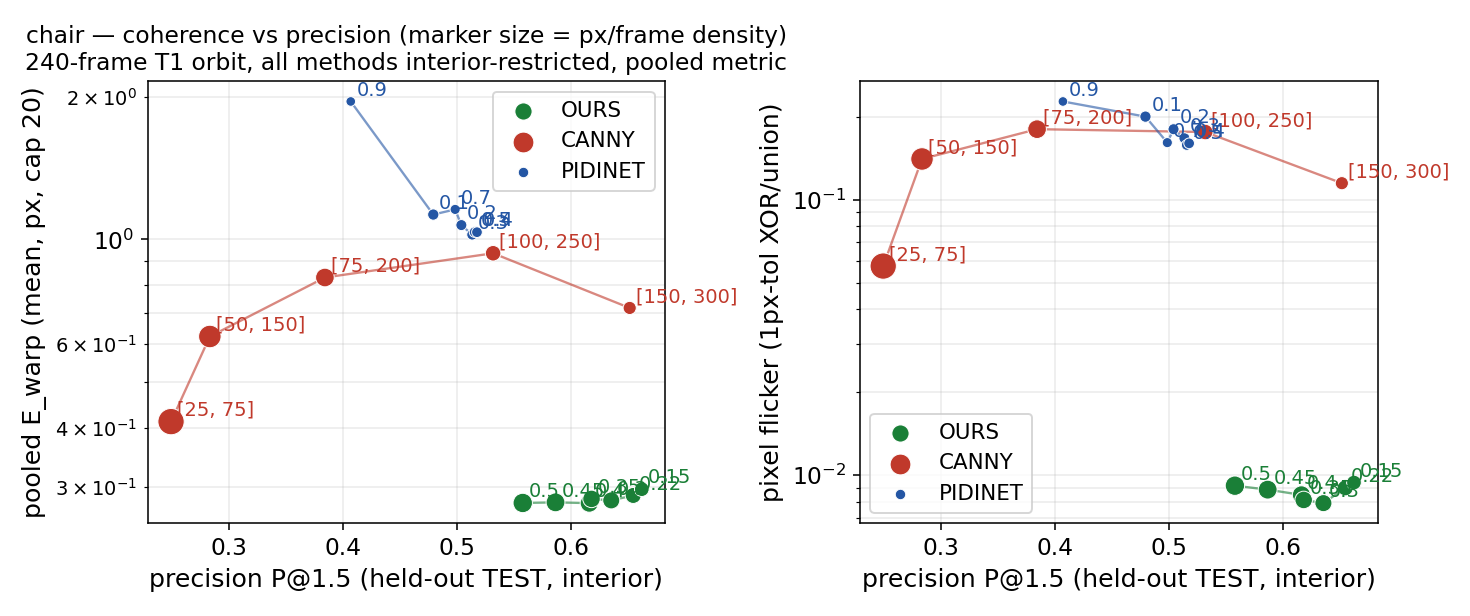
\includegraphics[width=\textwidth]{assets/pareto_chair.png}\\(a) chair\end{minipage}\hfill\begin{minipage}{0.465\textwidth}\centering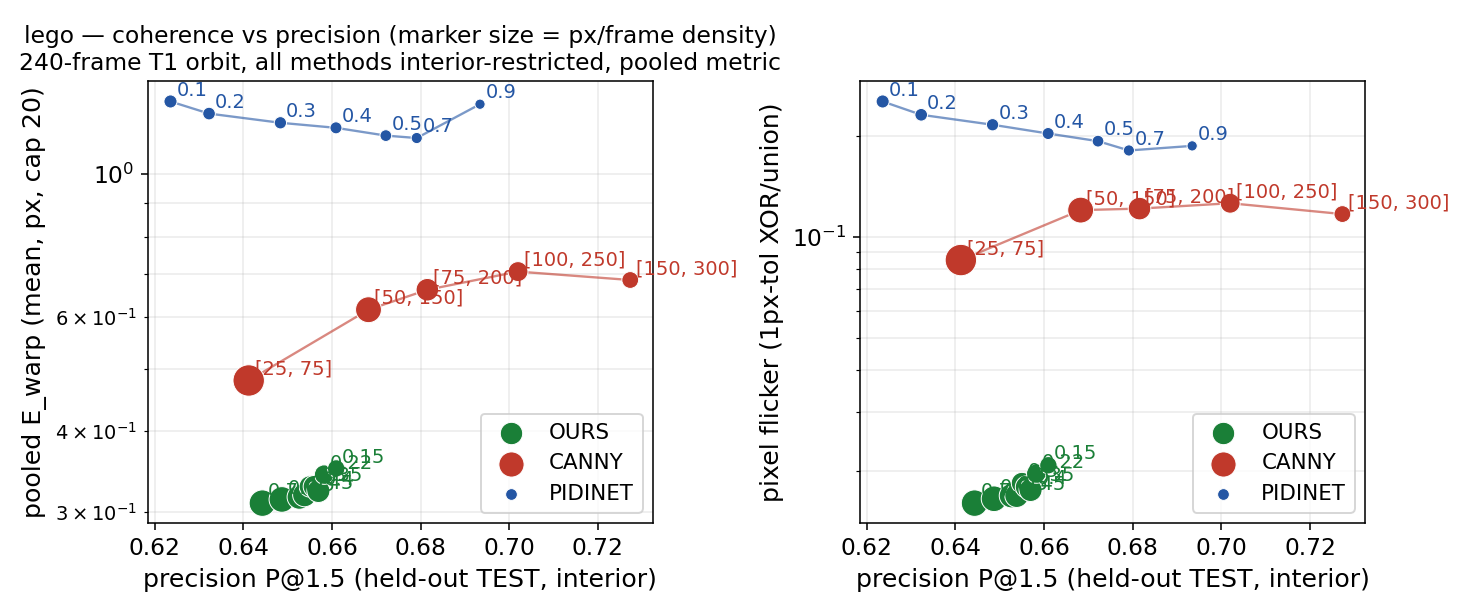
\includegraphics[width=\textwidth]{assets/pareto_lego.png}\\(b) lego\end{minipage}\caption{PARETO-1 precision/line-density operating frontiers: (a) chair, (b) lego.}\label{fig:2}\end{figure*}
\emph{(Contribution A, primary. All numbers from \texttt{RESULTS\_MASTER.md}; figures Fig.~\ref{fig:2}--5, Tab.~\ref{tab:1}--2.)}

\subsection{Protocol: three axes, one dominance rule}
A temporal-stability claim for a line primitive is easy to fake and easy to dismiss: a
method can look stable by drawing fewer lines or blurrier lines. Our protocol closes
those doors --- precision and pixel-density are matched jointly --- but we name what it does
not close: matched density is not matched \emph{coverage} (\S5.1 shows creases with no carrier
at all, which our lines cannot ink at any density), so the comparison certifies stability
of what is drawn, not equivalence of what is drawable. Every method --- ours and every baseline --- is swept
over its acceptance threshold to trace an operating curve over three axes: precision
(P@1.5 against held-out GT creases), line density (rendered line-pixels per frame), and a
pixel-pooled stability statistic. Stability is compared \textbf{only at shared operating
points}: a baseline point counts iff some point of ours matches or beats it on \emph{both}
precision and density; the reported advantage is the \emph{minimum} ratio over all such
dominating points. The stability statistic itself is pooled per pixel, not per line: every
ON line-pixel of frame \emph{t} is forward-warped by the exact rigid flow (rendered depth plus
the two camera poses --- the same operator for every method), and the distance transform of
frame \emph{t+1}'s line mask is read at the landing pixel; distances are pooled over all 239
transitions of a 240-frame trajectory. There is no matching step and no per-line
normalization, so a vanished line is charged automatically, and a sparse "sticky" line set
cannot be flattered. All methods are restricted to the object interior ($\alpha$>0.5, eroded
2 px), which removes the silhouette warp-drop confound at source for everyone (warp-drop
$\leq$0.1 \% throughout).

\subsection{Against memoryless per-frame detection}
At every shared operating point on both scenes, our projected object-space lines flicker
\textbf{$\geq$9.8$\times$} less than per-frame Canny and PiDiNet (pixel flicker, 1 px-tolerant XOR/union;
Fig.~\ref{fig:2}). The more telling observation is \emph{how} the two families traverse their operating
curves: our pooled pop-rate is \textbf{invariant to the acceptance threshold} (P(d>2 px) stays
within 0.0042--0.0049 across the entire sweep on chair) --- stability is a property of the
object-space parameterization, not of which lines are kept --- while the per-frame
detectors \emph{destabilize} as they sparsify (PiDiNet at thr 0.9 pops 3$\times$ more than at 0.1).
One pre-registered gate in this comparison failed, and we report it rather than re-tune
it: the pooled-\emph{mean} statistic's advantage drops to \textbf{2.42$\times$} at the sparsest
high-precision Canny point, below our frozen 3$\times$ bar. The dissection (Tab.~\ref{tab:2}) shows why the
statistic, not the stability, collapses: our lines are static 3D polylines whose true
inter-frame drift is zero, so their pooled mean sits at the shared \textasciitilde{}0.28 px
rasterization/warp quantization floor (p95 = 1.00 px, threshold-invariant), and a mean
over a floor-dominated distribution compresses ratios at sub-pixel motion. The floor-free
statistics at the \emph{same} point read 12.8$\times$ (pop) and 12.2$\times$ (flicker). We quote pop and
flicker as primary and disclose the mean-statistic collapse.

\subsection{Against an oracle-flow temporally-accumulated ceiling}
\begin{figure}[t]\centering\setcounter{figure}{2}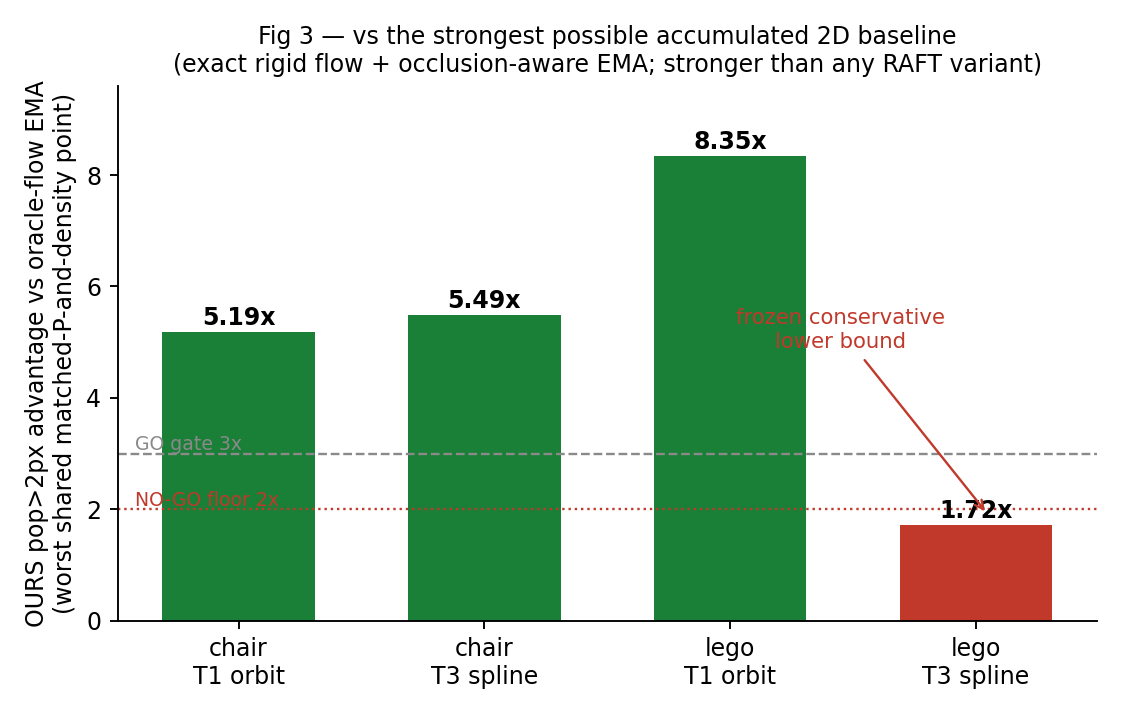
\includegraphics[width=\columnwidth]{assets/fig3_pareto2.png}\caption{Per-condition worst-case stability advantage against the oracle-flow accumulated baseline; the gate-breaching lego$\times$T3 cell is flagged as the reported floor.}\label{fig:3}\end{figure}
The strongest objection to \S4.2 is that per-frame detection is a strawman: a reviewer's
baseline would warp and accumulate edges over time. We therefore built the strongest
member of that family we know how to construct --- an EMA accumulator
(A\_t = $\alpha$$\cdot$warp(A\_\{t$-$1\}) + (1$-$$\alpha$)$\cdot$E\_t, rethresholded, $\alpha$ up to 0.85) driven by the \textbf{exact
rigid flow} with an occlusion-aware fallback, i.e. an oracle upper bound on every
estimated-flow variant --- and swept it on the same three axes (Fig.~\ref{fig:3}); the oracle claim covers the flow \emph{input}
only --- we make no claim over accumulator designs beyond this EMA family. Accumulation
genuinely helps the 2D baselines. It does not close the gap on the pooled pop-rate
P(d>2 px) --- the floor-free statistic \S4.2 motivates: the worst shared advantage per
condition is \textbf{5.19$\times$} (chair$\cdot$orbit), \textbf{5.49$\times$} (chair$\cdot$spline), \textbf{8.35$\times$} (lego$\cdot$orbit),
and \textbf{1.72$\times$} (lego$\cdot$spline); \S4.4 decomposes where this advantage lives and how much of
the baseline's residual is its own accumulator drift. The shared operating points sit at
P@1.5 0.28--0.59 on chair (9 and 8 of 21 baseline points shared) and 0.62--0.64 on lego (3
and 5 of 21) --- on lego the baseline's highest-precision configurations are not dominated by any
of our points and are therefore outside the comparison, a truncation the dominance rule
imposes by construction and we report rather than hide. The last cell breaches our frozen 2$\times$ bar and
we keep it as the headline of this subsection rather than a footnote: \textbf{1.72$\times$ is the
reported floor of the claim --- a breached pre-registered gate, not a designed margin} ---
measured against a baseline whose flow input no practical system can exceed, in the
single condition that maximizes occlusion flux.

\subsection{The operational envelope}
Where does the advantage live, and where does it stop? Decomposing the worst cell by
region (Fig.~\ref{fig:4}): the advantage is \textbf{interior} --- pop-rate 0.0214 vs the accumulator's
0.0425 (\textbf{1.98$\times$}) over the 93--97 \% of line-pixels away from occlusion boundaries --- and it
\emph{reverses} inside disocclusion regions, where our rate (0.407) is worse than the
baseline's (0.300): our visibility test splits chains at occlusion boundaries and the run
endpoints shift. We disclose this rather than a reviewer discovering it. A pre-registered
mechanism gate --- "$\geq$60 \% of the accumulator's residual popping lies in disocclusion
regions" --- came back \textbf{33.3 \%} (NO-GO): the accumulator's residual is diffuse interior
EMA drift, not a disocclusion-correspondence failure, so this paper makes \textbf{no}
mechanism claim about \emph{why} 2D accumulation trails; the bound is empirical. The envelope
is nonetheless predictable: the single sub-2$\times$ cell is exactly the condition (micro-relief
geometry $\times$ non-uniform multi-axis motion) where per-frame line-pixel turnover is dominated
by occlusion-boundary churn.

\subsection{Stroke-level corroboration}
\begin{figure*}[t]\centering\setcounter{figure}{4}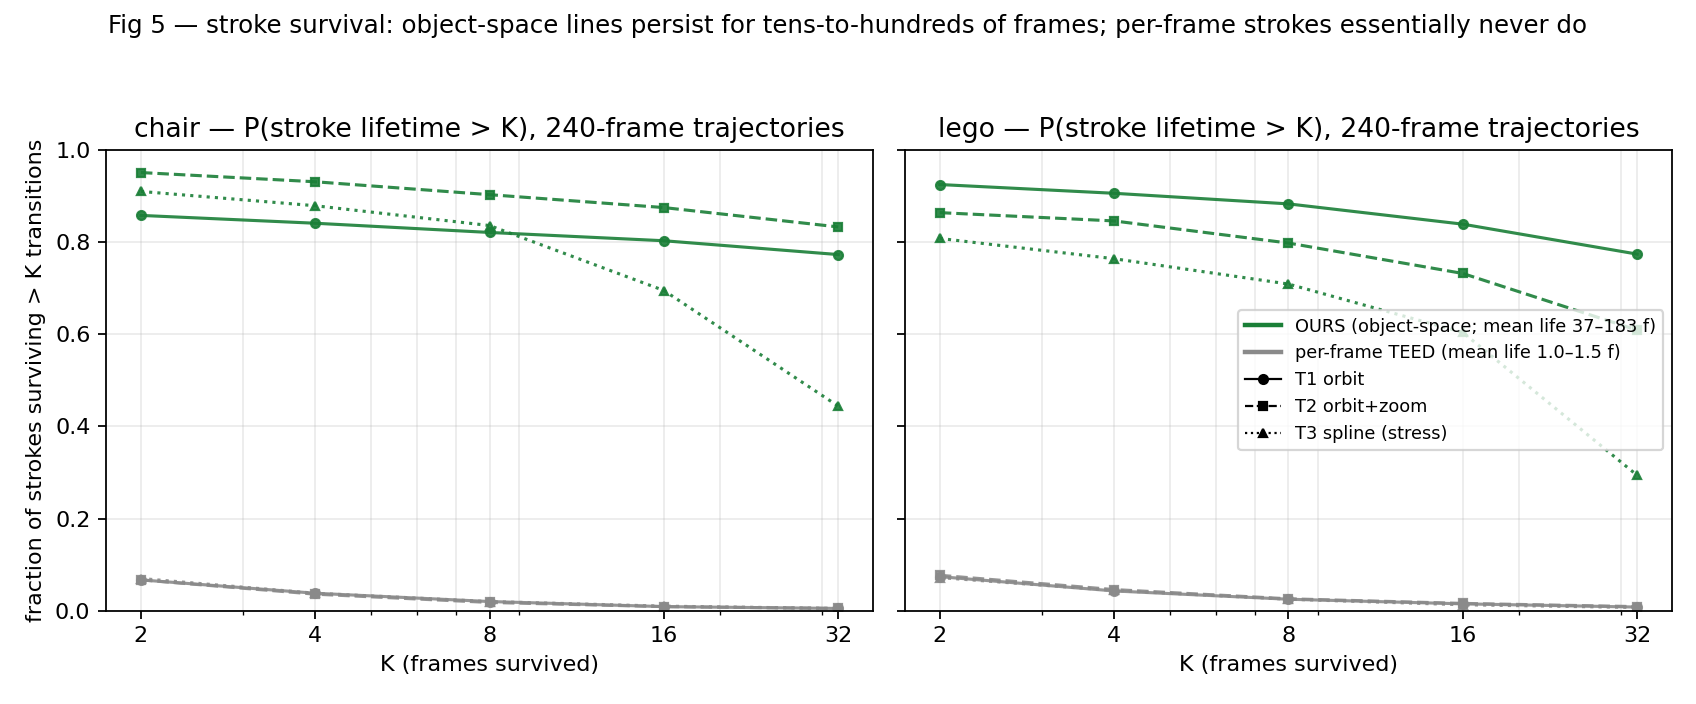
\includegraphics[width=0.53\textwidth]{assets/fig5_survival.png}\caption{Stroke-survival curves P(life${}>{}$K) for the six scene$\times$trajectory conditions: object-space strokes persist for tens-to-hundreds of frames; per-frame strokes essentially never do.}\label{fig:5}\end{figure*}
The pixel-pooled results above are corroborated by the independently built stroke-level
harness (Tab.~\ref{tab:1}, Fig.~\ref{fig:5}): matched-stroke E\_warp ratios of \textbf{3.38--21.62$\times$} across 2 scenes $\times$
3 trajectories against per-frame TEED (scorer and thresholds hash-frozen before any number
existed), Fr\'echet ratios of 2.43--29.92$\times$ against per-frame Canny, and --- most legibly ---
stroke \emph{survival}: object-space strokes persist for 37--183 frames on average where
per-frame strokes persist for 1.0--1.5 (P(lifetime>32): 0.29--0.83 vs 0.005--0.009). Our
stroke residual falls in proportion to per-frame motion, i.e. it is warp-resampling error
and nothing else; the per-frame baselines saturate at a motion-independent popping floor.
Fig.~\ref{fig:9} shows that comparison directly across the whole frame sweep together with both of its
confound controls --- the sparsity check and the silhouette warp-drop control --- and Tab.~\ref{tab:5}
collects the per-scene accuracy and coherence figures in one place.
These stroke-level harnesses predate the accumulated baseline and compare against
memoryless detection only; the oracle accumulator exists only in the pixel-pooled
protocol, so the third trajectory is covered at stroke level but not against
accumulation.

\emph{(Scope reminder for the section header: frozen 3DGS, static NeRF-synthetic scenes, known
poses; see \S6. The precision these curves operate at is itself bounded --- \S5 characterizes
that boundary.)}

\section{The precision boundary: a four-act characterization}
\begin{figure*}[t]\centering\setcounter{figure}{5}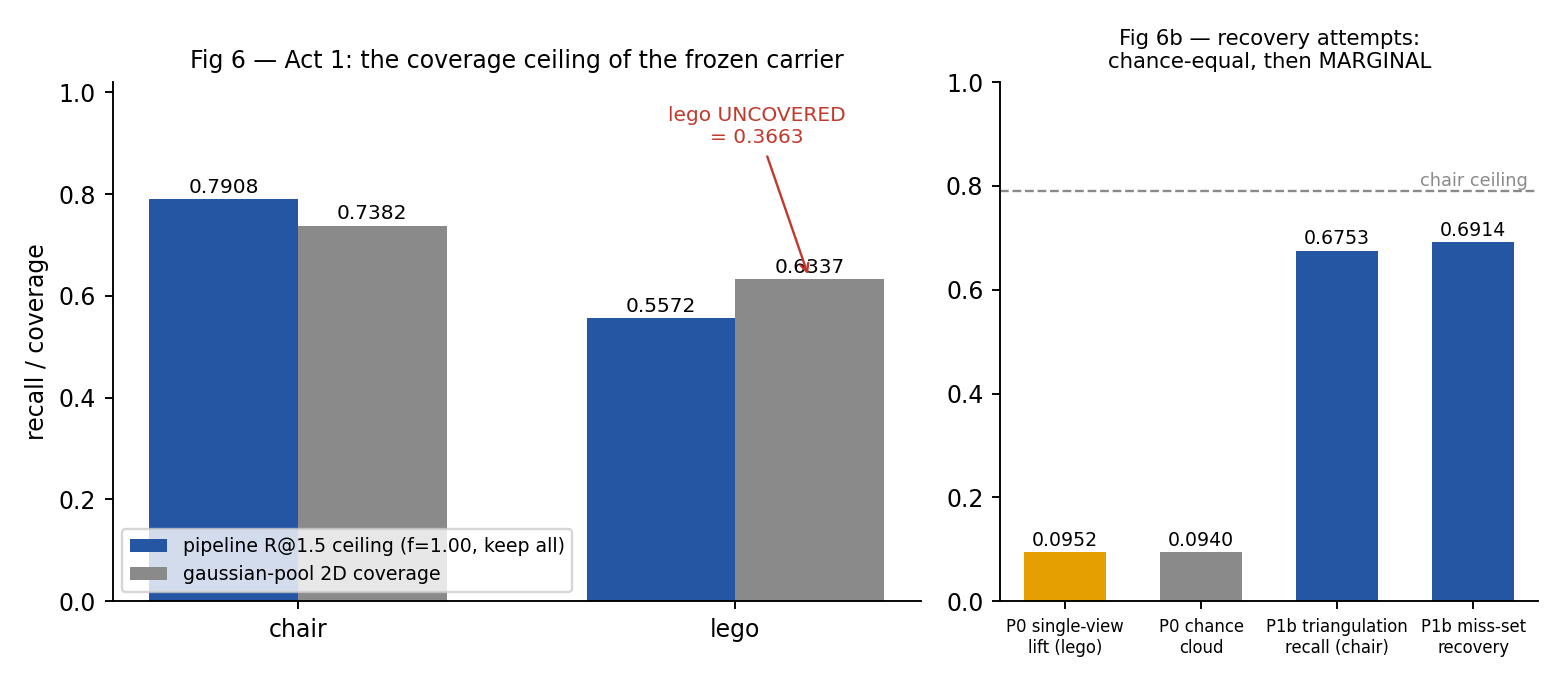
\includegraphics[width=0.66\textwidth]{assets/fig6_ceiling.png}\caption{Act 1: the carrier coverage ceiling, and the recovery ladder from single-view lifting to multi-view triangulation.}\label{fig:6}\end{figure*}
\emph{(Contribution B, diagnostic. All numbers from \texttt{RESULTS\_MASTER.md}; Fig.~\ref{fig:6}--8, Tab.~\ref{tab:3}--4.
Throughout, the GT mesh labels and scores only --- it never enters the method path.)}

\subsection{Act 1 --- the ceiling exists, and what it does and does not mean}
The primitive of \S4 operates at a bounded precision, and the bound begins with coverage:
re-ranking the frozen gaussian pool --- keeping \emph{everything} --- caps pipeline recall at
R@1.5 = 0.7908 (chair) / 0.5572 (lego); the pool's own 2D point coverage is 0.7382 /
0.6337 --- on chair the pipeline's recall exceeds point coverage because rasterized segments
interpolate \emph{between} carriers, so the binding form of the ceiling is lego's, where 0.3663
of visible GT crease points have no carrier within 1.5 px at all and interpolation cannot
manufacture one (Fig.~\ref{fig:6}).

Both figures are stated at the crease definition we use throughout --- mesh edges whose dihedral
angle exceeds a fixed threshold --- and lego is unusually sensitive to that choice, so we report
the sensitivity rather than leave it implicit. lego's mesh contains a single large family of
edges lying at exactly the threshold angle, which the threshold splits near-evenly through the
asset's six-decimal vertex quantisation; nudging the threshold by a twentieth of a degree
therefore discards nearly half of lego's crease pixels and raises the measured ceiling
materially, after which it plateaus. This is a property of the asset, not of the reconstruction
or of the extractor, and it does not describe a better pipeline: precision over the identical
rasterised segments falls by more than half across the same range, F-score is flat-to-declining,
and the joint operating gate is met at no threshold on either scene. chair, which carries no such
family, is unaffected. The ceiling conclusion is therefore robust to the threshold even though
the individual number is not; the per-threshold values are tabulated in the results ledger.
Some of those uncovered creases are flat decals with literally zero geometric footprint.

This admission invites a specific attack, so we answer it here rather than in a rebuttal:
\emph{if the lines live on a baked radiance carrier, is \S4's stability just the passive
reprojection of 2D edges --- an inherited artifact that this ceiling proves?} Not on the
evidence --- though the evidence is single-scene, as \S6 states plainly. On the texture-bound scene,
the carrier surface under a high-contrast fabric edge is indistinguishable from the
carrier under a crease --- on this population the fabric-bound rows of Act 2 apply directly
(the albedo-step gate leaks, 0.1235 vs 0.1211, and multi-view consistency does not
separate, 0.870 vs 0.937), and the geometric cues of Tab.~\ref{tab:3} are at or below chance on the
decisive decal population --- yet our extracted set is substantially \textbf{more precise than the photometric edge field
itself} --- P@1.5 0.662 at 4,947 px/frame vs per-frame Canny 0.532 at 5,973 px/frame, and,
in the dominance-consistent direction (ours denser AND more precise), 0.636 at 7,942
px/frame vs the same 0.532 (Fig.~\ref{fig:2}): the pipeline actively \textbf{suppresses} texture edges that enjoy the
same carrier support and the same image contrast as the creases it keeps. That is genuine
multi-view selectivity performed by the object-space aggregation --- work the carrier could
not have done for us (Act 2) and the 2D edge field did not do for us (Fig.~\ref{fig:2}) --- not passive
reprojection. The converse case gets equal prominence: on lego, where strong image edges
largely \emph{are} creases, per-frame Canny is more precise than our lines at every density;
there our advantage is stability only. The ceiling, then, bounds \emph{which} creases
the primitive can carry --- it says nothing against \emph{how stably} it carries them, which is
\S4's claim and survives at matched precision and density.

\subsection{Act 2 --- no geometric cue separates the miss-set (K\_geom $\approx$ 0)}
Could a better geometric gate recover the uncovered creases or reject the texture? On the
decisive population (lego decals vs true creases), no geometric channel is usable (Tab.~\ref{tab:3};
several score \emph{below} chance --- decals locally out-score creases --- so even sign-flipped
they reverse the intended semantics): 2DGS surfel dihedral 0.4110, rendered-normal ribbons 0.3307/0.3875, and ---
the controlling result --- the \textbf{GT mesh's own dihedral, 0.3964}, with normal-dispersion
medians 44.52$^{\circ}$ vs 44.84$^{\circ}$: given \emph{perfect} geometry, the two classes differ by 0.32$^{\circ}$. The
low-level photometric escape routes close the same way: the SH-DC albedo-step gate leaks
(fabric p50 0.1235 vs crease 0.1211), and multi-view consistency does not separate
(texture 0.870 vs crease 0.937 --- printed patterns are rigid surface loci too). Coverage
recovery fares no better: single-view photometric lifting equals its chance control
(R\_miss 0.0952 vs 0.0940), and multi-view triangulation, though a genuine localization
fix, stays detector-bound at MARGINAL (recall 0.6753 / miss-set recovery 0.6914; Fig.~\ref{fig:6}b).

\subsection{Act 3 --- the separating signal exists}
The missing discriminator is not hiding in geometry; it is semantic. A linear probe on
frozen zero-shot DINOv2 features~\cite{dinov2} separates crease from texture at AUC \textbf{0.8401 / 0.9044}
(chair / lego, held-out spatial split), 0.8205 / 0.8913 under the leakage-guarded
chain-level read, against $\approx$0.71 photometric and $\approx$0.65 geometric probe baselines on the candidate
population --- a different population and feature set from \S5.2's decal test, which is why
a nonzero geometric number here does not contradict K\_geom$\approx$0 there (Fig.~\ref{fig:7}). Read
honestly, the probe recognizes \emph{which surface} a point lies on --- fabric field vs piping,
stud field vs decal --- a surface-identity readout rather than an edge-type detector. The
signal the primitive needs exists, in features every modern pipeline already has --- though
Act 4 shows that reading it out is supervision-bound.

\subsection{Act 4 --- and it is supervision-bound under our frozen protocol}
The signal exists (0.8401/0.9044) --- but it collapses under mesh-free supervision (Fig.~\ref{fig:8}): trained
on our best mesh-free pseudo-labels (physics-frozen geometric-photometric votes, and a
fully self-supervised clustering variant), the same probe falls to \textbf{0.6371} on chair
through a pre-registered 0.72 gate (on lego 0.9046 --- the ceiling as recomputed in this
study; 0.9044 in Act 3's split --- falls to 0.6569), beneath even its photometric baseline:
the best mesh-free number \emph{anywhere} is the chair photometric probe at 0.7326 --- touching
the gate on one scene, 0.5637 on the other --- while the semantic probe collapses on both. The failure mode is instructive: the pseudo-labels' errors are systematic, not
noisy, and the richer representation learns them the more faithfully --- zero denoising. One
route stays open, and we measured it: the mesh-supervised probe transfers chair$\rightarrow$lego at
\textbf{0.8245}, nearly matching lego's in-scene ceiling, though not in reverse (0.5626).
Precision is therefore \textbf{supervision-bound under our frozen protocol} --- with labeled
training scenes as the named, tested-in-one-direction path forward. Appendix A closes the
loop at deployment granularity: used as an actual gate on the line-candidate cloud, the
deployment-legal direction of that transfer (0.5626, chance) leaves precision untouched,
and even an in-scene mesh oracle cannot filter the cloud to the pipeline's precision
without severing crease connectivity.

\subsection{What the boundary buys}
This characterization is what licenses \S4's scope. The arc --- coverage bounded by the
carrier (5.1), the miss-set geometrically invisible (5.2), the discriminator semantic and
extant (5.3), its mesh-free readout falsified through a frozen gate (5.4) --- explains
\emph{why} we ship a stability primitive at a measured precision rather than patching precision
with an in-scene oracle: every patch we tested either equals chance, stays
detector-bound, requires supervision the method path is not allowed to touch, or --- when
granted that supervision as an explicit oracle --- fragments the very chains it is meant to
purify (Appendix A). The boundary is measured, disclosed, and has exactly one open door:
labeled scenes feeding a topology-aware construction, not a post-hoc filter.

\section{Limitations}
\emph{(All numbers from \texttt{RESULTS\_MASTER.md}. Nothing here is softened; several of these limits
were established by our own pre-registered gates coming back negative.)}

\textbf{In-vitro scope.} Everything in this paper is measured on frozen 3DGS reconstructions of
two static NeRF-synthetic scenes~\cite{nerf} with known poses and rendered depth --- an in-vitro
geometric characterization, owned as such rather than patched. Every baseline shares the
same perfect-geometry assumptions (the accumulated baseline is \emph{given} our exact rigid
flow), so the comparisons are internally fair, but n=2 synthetic scenes with perfect
geometry is the breadth we have; real captures, estimated poses, and more scenes are
future work, not implied results.

\textbf{The selectivity evidence is single-scene.} The \S5.1 demonstration that our pipeline
actively suppresses texture edges --- higher precision than its own seed edge field at
matched density --- holds on chair only. On lego, per-frame Canny is \emph{more precise than our
lines at every density we reach}; our advantage there is stability alone. Selectivity is
demonstrated on the texture-bound scene and not contradicted on the geometry-dense one.
The stability claim itself does not lean on this: \S4.1's dominance rule compares stability
only at operating points the baselines actually share on both precision and density, so
\S4's ratios survive on lego with no selectivity assumption at all.

\textbf{The temporal advantage is interior-only, and reverses at disocclusions.} Decomposing
the hardest cell (\S4.4): the entire advantage is interior EMA-drift suppression --- pop-rate
0.0214 vs the oracle accumulator's 0.0425, \textbf{1.98$\times$}, over the 93--97 \% of line pixels away
from occlusion boundaries --- while inside disocclusion regions \textbf{our method is worse}
(0.407 vs 0.300): visibility-culled chain runs split and their endpoints shift. Our
pre-registered mechanism gate ("$\geq$60 \% of the accumulator's residual lies in disocclusion
regions") came back \textbf{33.3 \%}, a NO-GO, so we claim \textbf{no} disocclusion-correspondence
mechanism for why 2D accumulation trails; the temporal bound is empirical.

\textbf{Precision is not solved --- it is supervision-bound.} The crease-vs-texture signal exists
in frozen DINOv2 features (0.8401/0.9044 with mesh labels) but collapsed to \textbf{0.6371}
under our best mesh-free supervision, through a pre-registered 0.72 gate (NO-GO). The one
measured route forward --- cross-scene transfer of a mesh-supervised probe --- works in one
direction of the two tested (0.8245 chair$\rightarrow$lego, 0.5626 reverse). Appendix A sharpens
this limit at deployment granularity: gating the line-candidate cloud with the
deployment-legal transfer probe converts nothing (precision 0.3216 vs 0.3189 ungated, at
matched recall), and even an in-scene mesh-oracle ranking cannot reach precision 0.71,
baseline recall, and crease connectivity 0.90 simultaneously --- post-hoc filtering is a
falsified repair class (cloud-level probes: chair only, n=1; Appendix A). To pre-empt
the reading that this falsification merely benchmarked a pathological scene: chair is the
\emph{selected} texture-stress adversary (Canny edge purity 0.28 --- most of its edge field is
not crease), the two barriers are mechanistic rather than chair-specific (a supervision
gap that is transfer-asymmetric by measurement, and bridge-point severing that follows
from thresholding any fixed candidate set), and extending the falsification to more
scenes is named future work, not an implied result. Any deployment needing crease-level precision on textured
surfaces currently needs labeled scenes --- and, per Appendix A, a topology-aware
construction rather than a filter to spend them on.

\textbf{Geometry cannot rescue it (K\_geom $\approx$ 0).} This is not an artifact of our reconstruction:
even the \textbf{GT mesh's own dihedral scores AUC 0.3964} on crease-vs-decal, with
normal-dispersion class medians 0.32$^{\circ}$ apart. On decal-like structure there is no geometric
signal to find, for any method that seeds on geometry.

\textbf{Coverage is ceiling-bound.} Re-ranking the frozen carrier caps recall at R@1.5 =
\textbf{0.7908 (chair) / 0.5572 (lego)}; on lego \textbf{0.3663} of visible GT crease points have no
carrier within 1.5 px at all (flat decals prominent among them). Our lines cannot draw
what the carrier never represented, and \S5.2 shows the recovery attempts we falsified.

\textbf{Further disclosed limits, collected.} Four limits disclosed elsewhere belong in this
list too: all pipeline constants were selected during development with mesh-scored
validation views (\S3.4); the pooled-\emph{mean} stability statistic failed its own 3$\times$ gate at
one point (2.42$\times$, \S4.2); no third-party static-curve method was compared (\S2, an
evaluation boundary); and the shared operating points on lego sit at P@1.5 $\approx$ 0.63 with the
baseline's highest-precision configurations excluded by the dominance rule (\S4.3).

\textbf{Evaluation dependency.} GT supervision (crease labels, precision/recall scoring) comes
from the mesh, confined to \texttt{mesh\_oracle.py} and the eval scripts --- the method path never
imports it (AST-verified per phase). The flip side of this hygiene: our quantitative
evaluation is only available where GT meshes exist, which is part of why the study is
in-vitro.

\section{Conclusion}
We set out to extract clean, temporally stable 3D feature lines from a frozen 3DGS, and we
report exactly what that produced --- two contributions, each scoped to what was measured.

\textbf{A stability finding.} Object-space feature lines whose rendered strokes are
\textbf{1.72--8.35$\times$} more temporally stable per condition than an oracle-flow temporally
accumulated 2D baseline --- \textbf{5.19$\times$ or better in three of four scene$\times$trajectory conditions;
the 1.72$\times$ stress-spline cell breached its pre-registered 2$\times$ bar and stands as the reported
floor} --- and $\geq$9.8$\times$ more stable than memoryless per-frame detection, at matched precision
\emph{and} matched line density, on n=2 synthetic scenes and at precision bounded by the second
contribution (mesh-free discriminability 0.6371 AUC). The stability is invariant to the
acceptance threshold across the chair sweep (not repeated on lego),
consistent with it being a property of the object-space parameterization rather than of
line selection. The claim ships with its measured envelope: the advantage is interior
(1.98$\times$), reverses inside disocclusion regions, and is valid for frozen reconstructions of
static scenes with known poses.

\textbf{A boundary forensics.} The primitive's precision is \emph{not} solved --- the four-act
characterization of why is itself a contribution: coverage is capped by the frozen carrier
(0.7908/0.5572); the missing creases carry no geometric signal even under the GT mesh
(AUC 0.3964); the discriminating signal exists in frozen semantic features (0.8401/0.9044)
--- and collapses under mesh-free supervision through a pre-registered gate (0.6371 vs a
0.72 bar), leaving cross-scene transfer (0.8245, one direction) as the tested route
forward --- and the patch family itself is falsified: no tested post-hoc filter of the candidate
cloud --- mesh-free or oracle-ranked, point- or chain-pooled --- reached the pipeline's
precision at matched recall with crease connectivity intact (the topological trilemma,
Appendix A). Precision on textured surfaces is supervision-bound under our frozen
protocol; we ship the boundary, measured, rather than a patch.

Methodologically, every gate in this study was frozen before its numbers existed and
evaluated on its letter (the full ledger is Tab.~\ref{tab:4}); the unfavorable outcomes --- including the two failed stability
gates and the supervision-bound NO-GO --- are reported with the same prominence as the
favorable ones, because several of this paper's most useful sentences (the quantization
floor, the disocclusion reversal, the oracle-baseline gap) exist only because a failed
gate was dissected instead of defended. We believe the resulting object --- a stability
primitive with a measured boundary --- is more useful to build on than either an
undisclosed-limit system or an unmeasured negative.



\clearpage
\begin{thebibliography}{9}
\bibitem{kerbl3dgs} B.~Kerbl, G.~Kopanas, T.~Leimk\"uhler, and G.~Drettakis.
3D Gaussian splatting for real-time radiance field rendering.
\emph{ACM Trans.\ Graph.\ (SIGGRAPH)}, 2023.
\bibitem{canny1986} J.~Canny. A computational approach to edge detection.
\emph{IEEE TPAMI}, 1986.
\bibitem{dexined} X.~Soria, E.~Riba, and A.~Sappa. Dense extreme inception network:
Towards a robust CNN model for edge detection. In \emph{WACV}, 2020.
\bibitem{teed} X.~Soria, Y.~Li, M.~Rouhani, and A.~Sappa. Tiny and efficient model for
the edge detection generalization. In \emph{ICCV Workshops}, 2023.
\bibitem{pidinet} Z.~Su, W.~Liu, Z.~Yu, D.~Hu, Q.~Liao, Q.~Tian, M.~Pietik\"ainen, and
L.~Liu. Pixel difference networks for efficient edge detection. In \emph{ICCV}, 2021.
\bibitem{dinov2} M.~Oquab et~al. DINOv2: Learning robust visual features without
supervision. \emph{TMLR}, 2024.
\bibitem{emap} L.~Li, S.~Peng, Z.~Yu, S.~Liu, R.~Pautrat, X.~Yin, and M.~Pollefeys.
3D neural edge reconstruction. In \emph{CVPR}, 2024.
\bibitem{sketchsplat} H.~Ying and M.~Zwicker. SketchSplat: 3D edge reconstruction via differentiable multi-view sketch splatting. arXiv preprint arXiv:2503.14786, 2025.
\bibitem{nerf} B.~Mildenhall, P.~P. Srinivasan, M.~Tancik, J.~T. Barron,
R.~Ramamoorthi, and R.~Ng. NeRF: Representing scenes as neural radiance fields for view
synthesis. In \emph{ECCV}, 2020.
\end{thebibliography}

\section*{Supplementary figures and tables}
\noindent\emph{Referenced from the main text; numbering matches the in-text references.}

\begin{table*}[t]\centering\setcounter{table}{0}\caption{Matched-stroke E-warp ratios across scenes, trajectories and detectors.}\label{tab:1}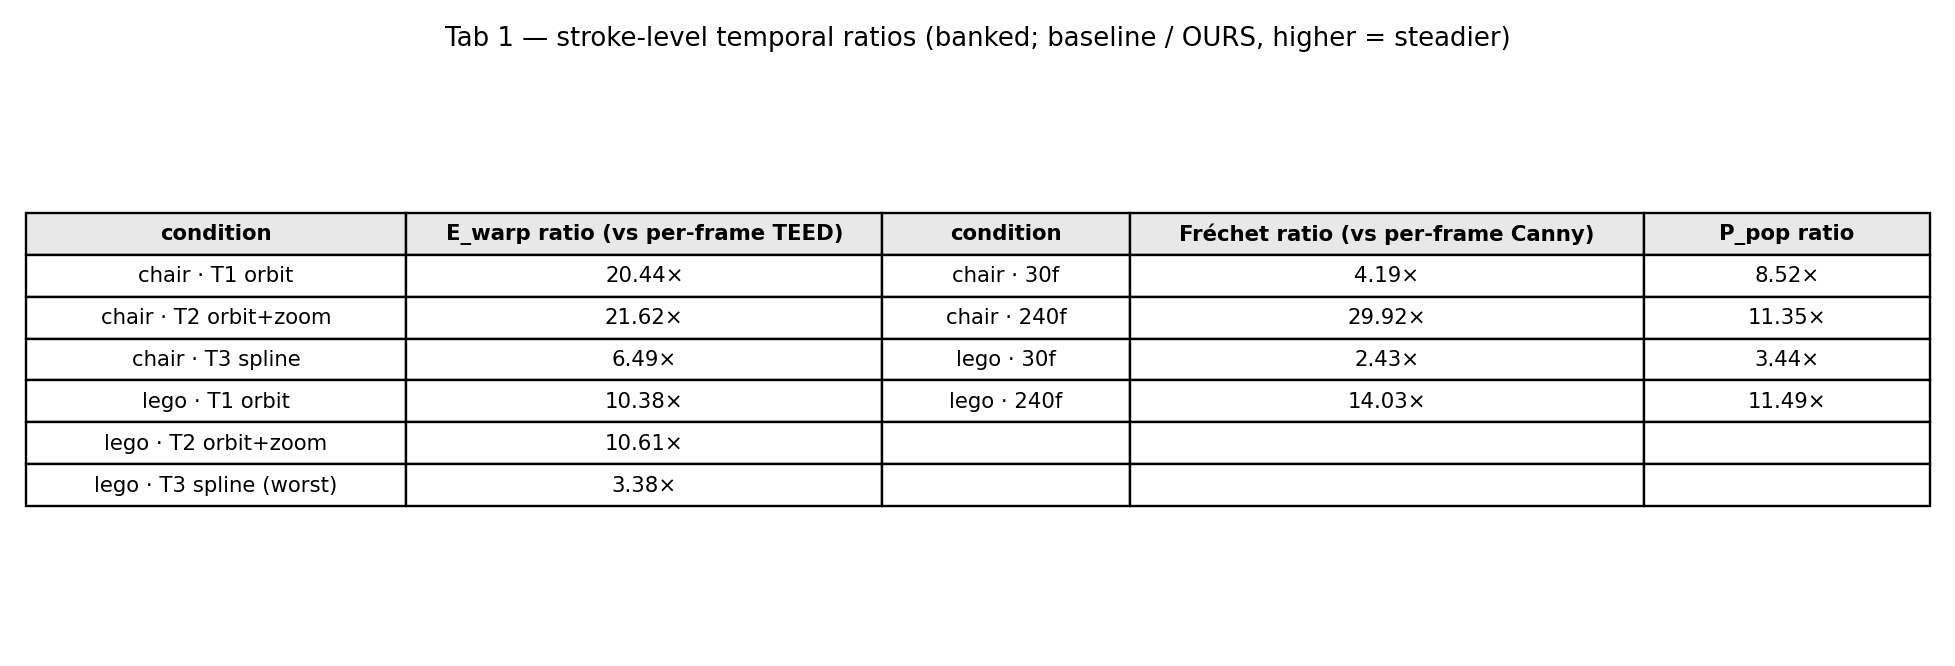
\includegraphics[width=0.8\textwidth]{assets/tab1_stroke_ratios.png}\end{table*}
\begin{table*}[t]\centering\setcounter{table}{1}\caption{Floor anatomy of the pooled-mean statistic.}\label{tab:2}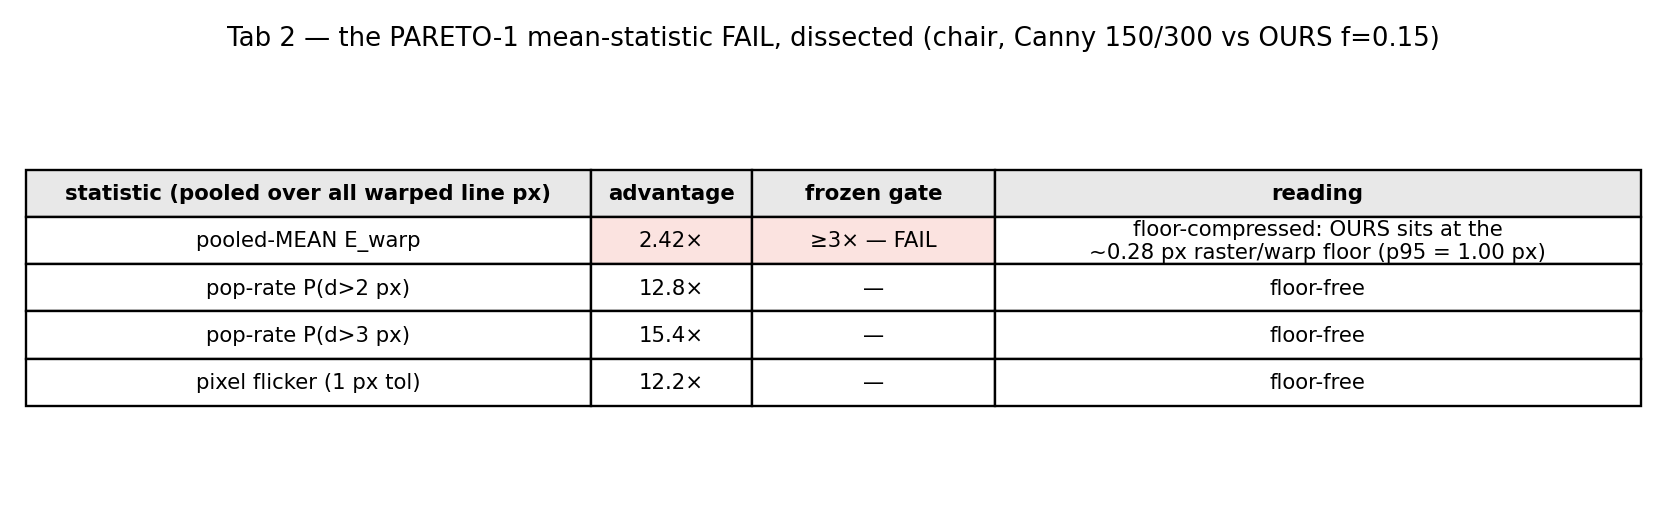
\includegraphics[width=0.62\textwidth]{assets/tab2_floor_anatomy.png}\end{table*}
\begin{table*}[t]\centering\setcounter{table}{2}\caption{K\textsubscript{geom}: geometric cues on the miss-set.}\label{tab:3}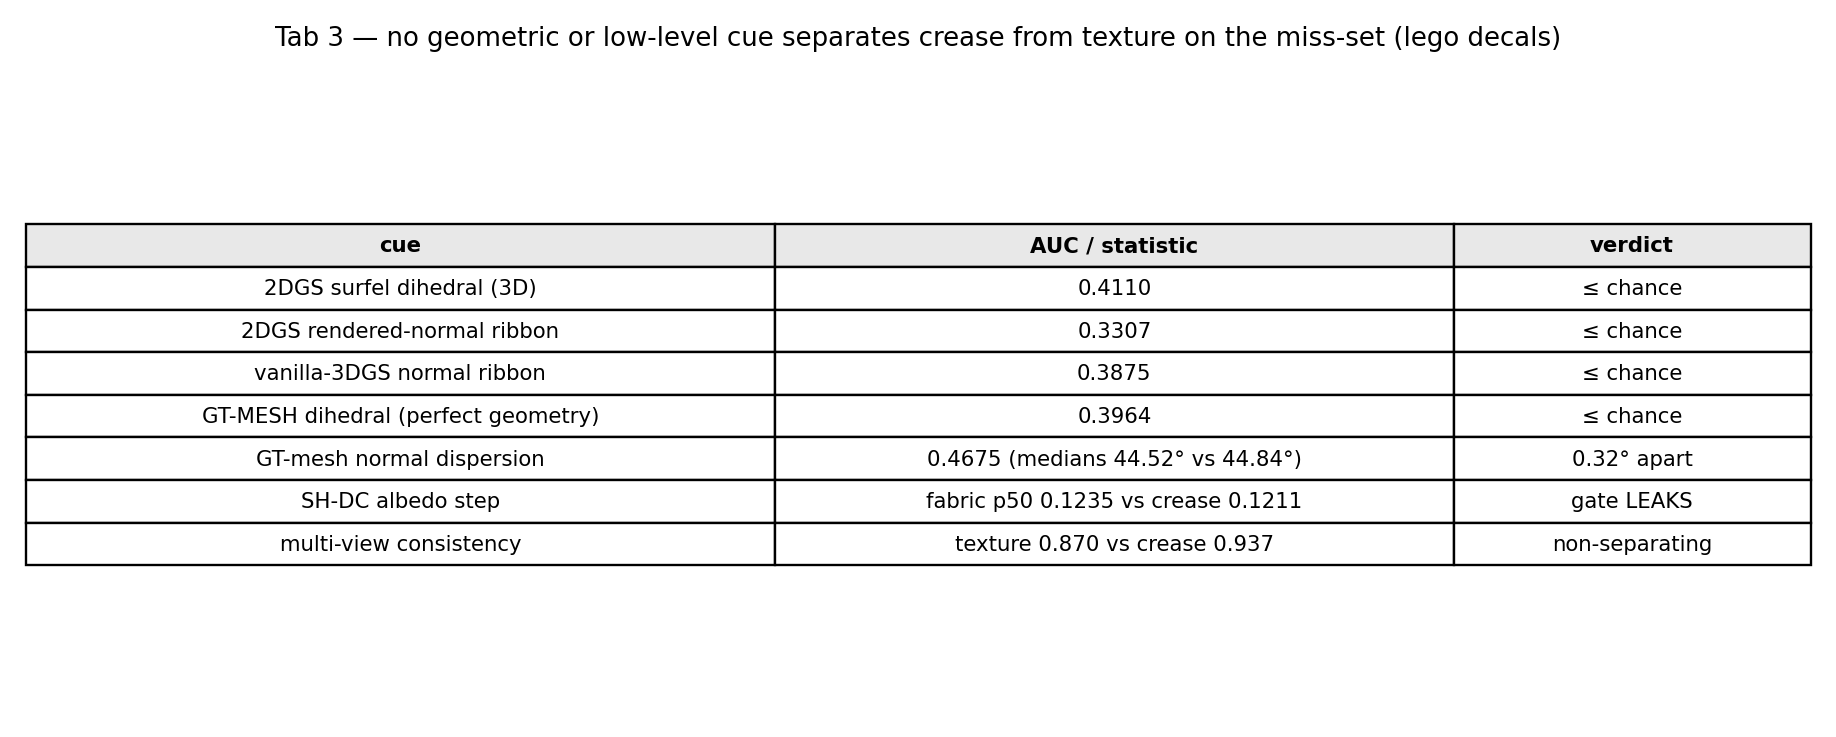
\includegraphics[width=0.55\textwidth]{assets/tab3_kgeom.png}\end{table*}
\begin{table*}[t]\centering\setcounter{table}{3}\caption{The frozen-gate ledger: every pre-registered gate, its bar, its measured value, and its disposition.}\label{tab:4}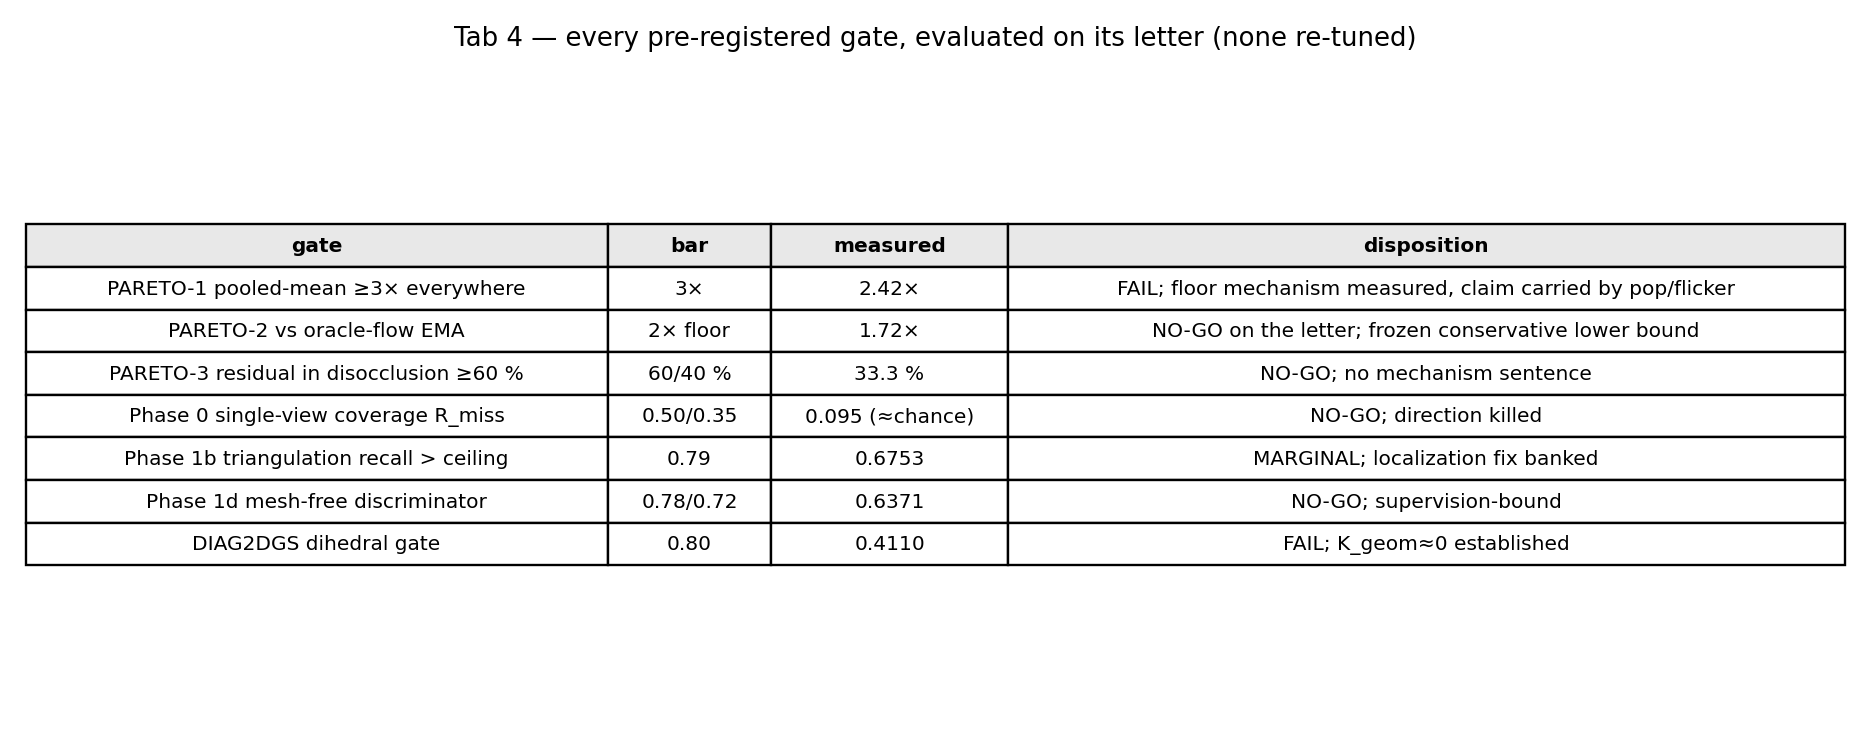
\includegraphics[width=0.62\textwidth]{assets/tab4_gate_ledger.png}\end{table*}
\begin{figure*}[t]\centering\setcounter{figure}{3}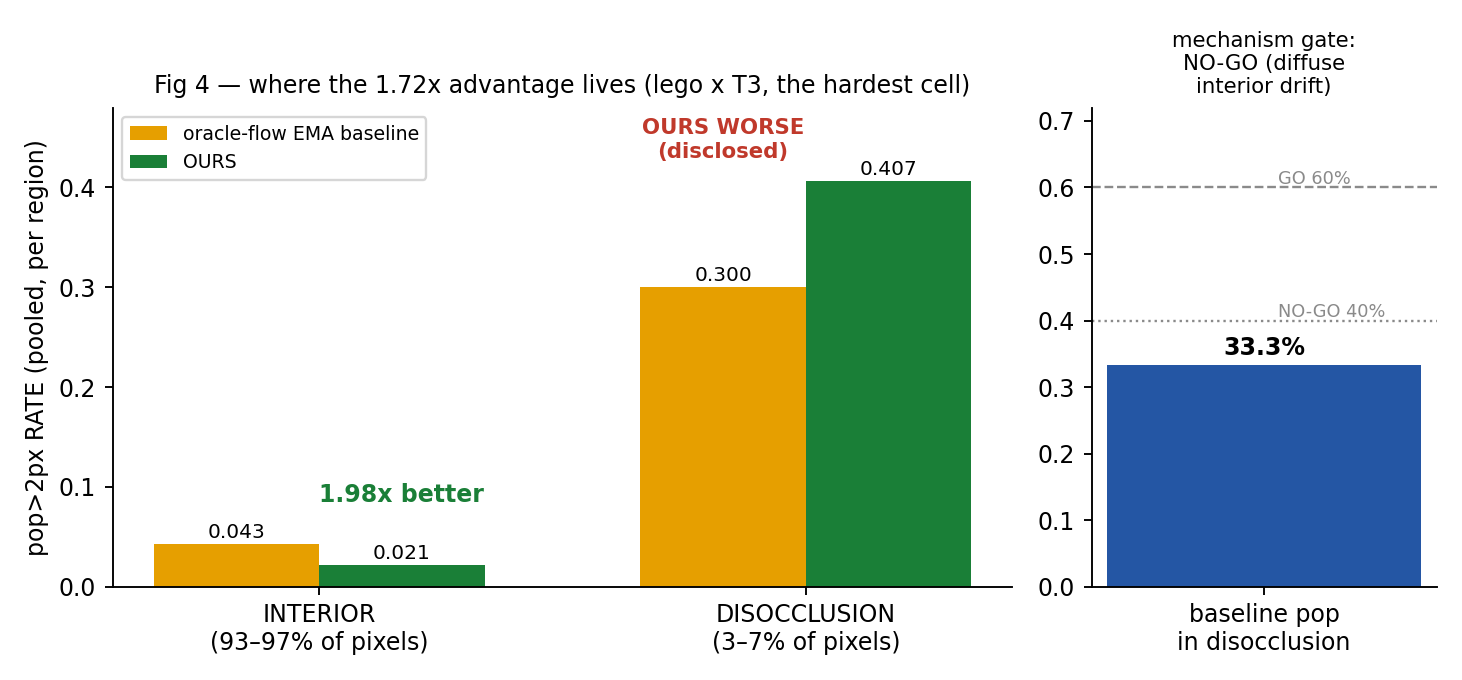
\includegraphics[width=0.75\textwidth]{assets/fig4_pareto3.png}\caption{Disocclusion decomposition of the hardest cell: the advantage is interior, reverses inside disocclusion regions, and the mechanism gate lands NO-GO.}\label{fig:4}\end{figure*}
\begin{figure*}[t]\centering\setcounter{figure}{6}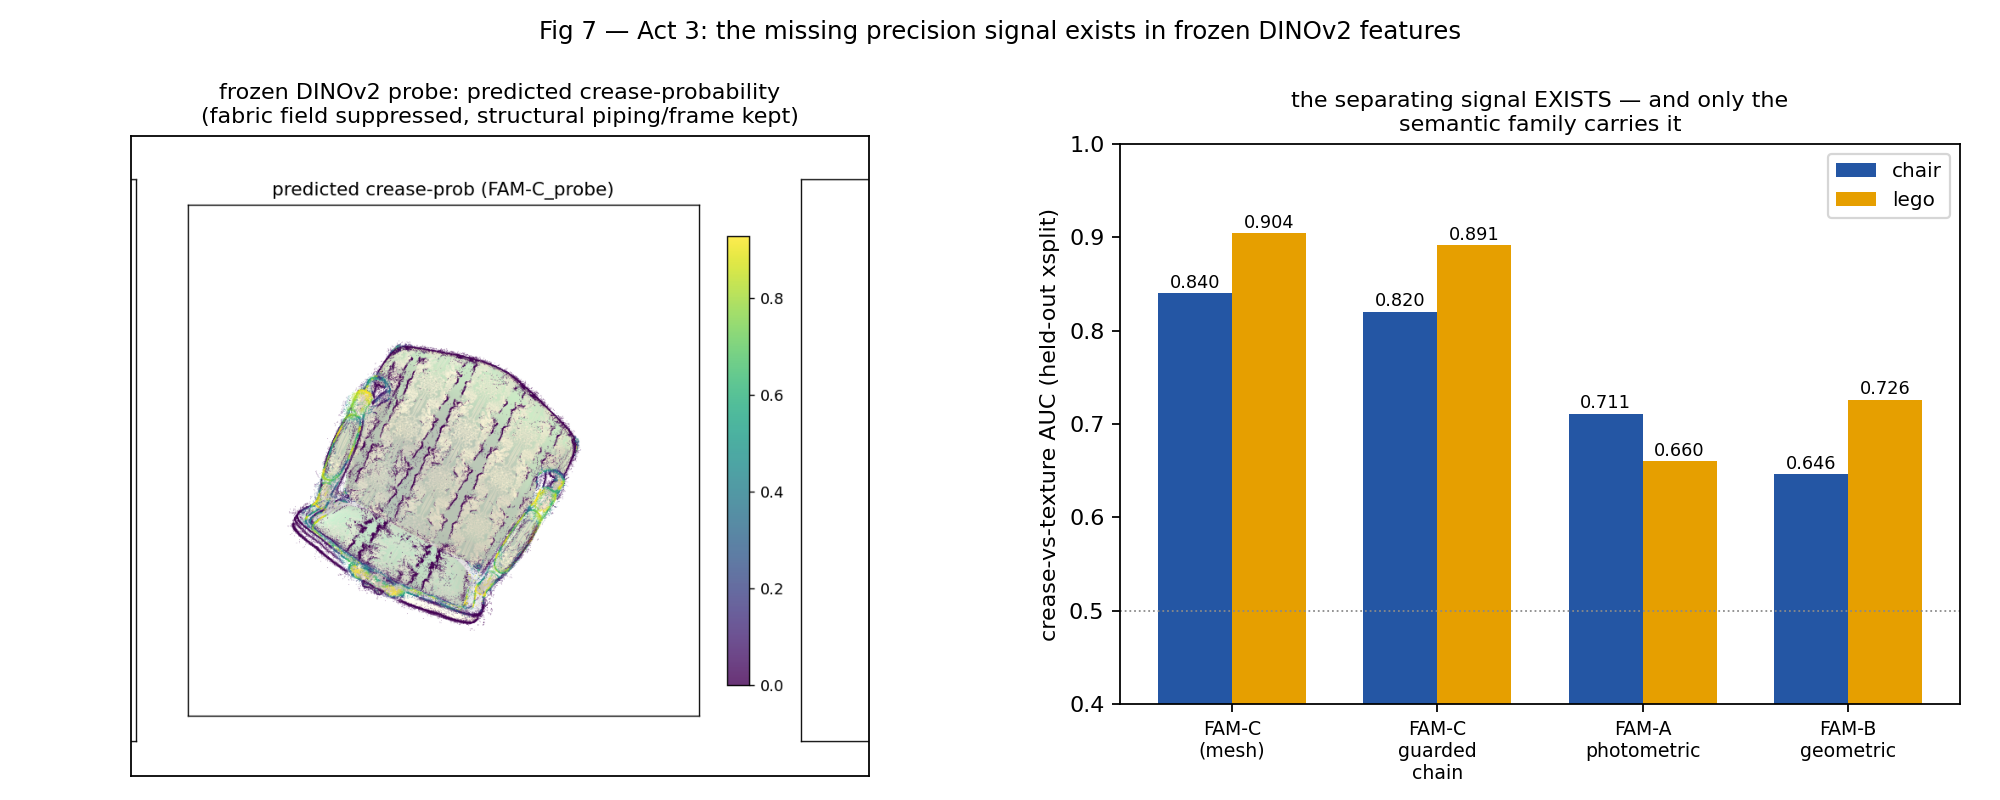
\includegraphics[width=0.85\textwidth]{assets/fig7_semantic.png}\caption{Act 3: frozen-DINOv2 crease-probability read-out and probe AUCs.}\label{fig:7}\end{figure*}
\begin{figure*}[t]\centering\setcounter{figure}{7}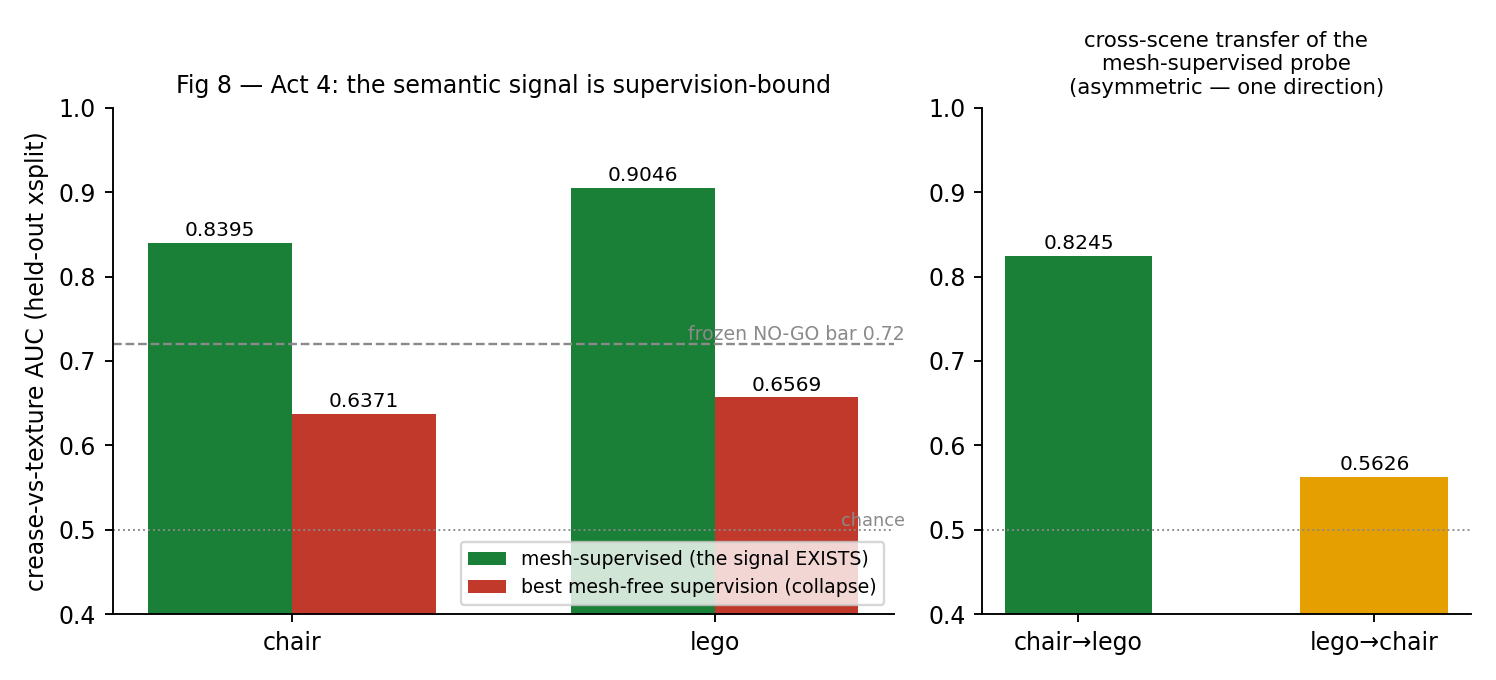
\includegraphics[width=0.75\textwidth]{assets/fig8_supervision.png}\caption{Act 4: the mesh-free supervision collapse, and the asymmetric cross-scene transfer. The mesh-supervised bars show the ceilings as recomputed in the falsification study; they agree with Act 3's split values quoted in the text to the third decimal.}\label{fig:8}\end{figure*}
\begin{figure*}[t]\centering\setcounter{figure}{8}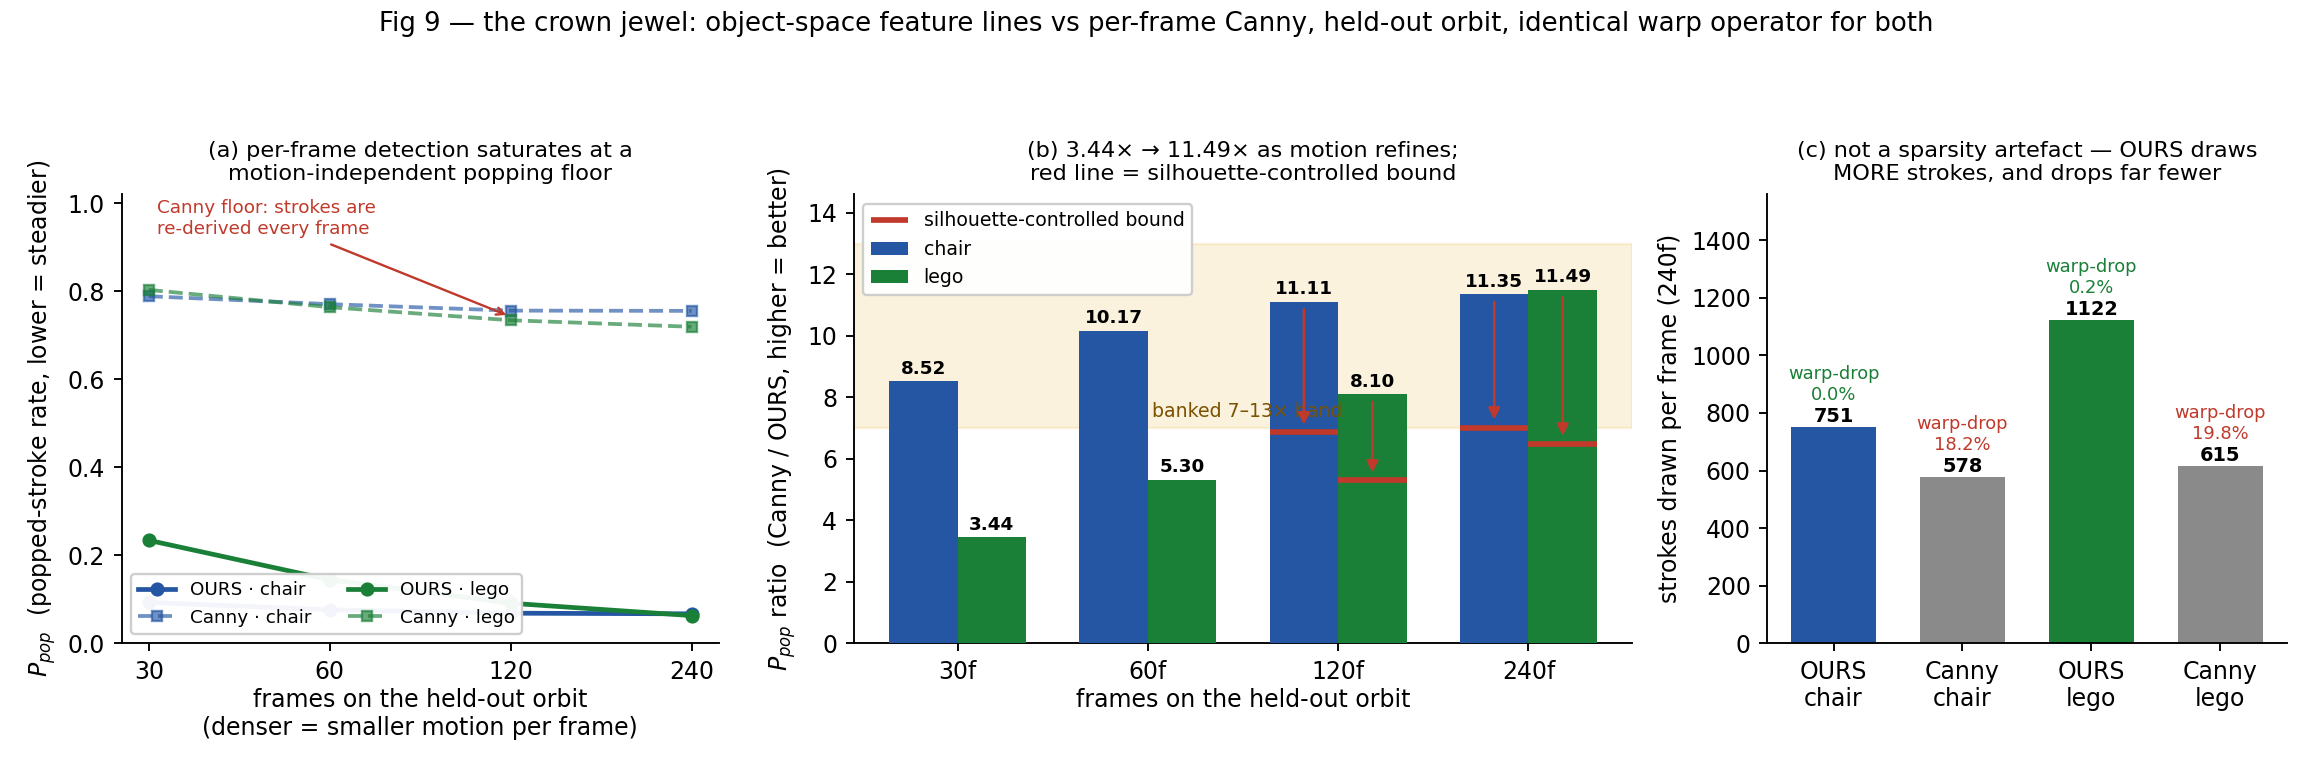
\includegraphics[width=0.98\textwidth]{assets/fig9_crownjewel.png}\caption{Object-space feature lines versus per-frame Canny on a held-out orbit, under an identical forward-warp operator for both pipelines. Left: per-frame detection saturates at a motion-independent popping floor while object-space strokes fall in proportion to the per-frame motion. Centre: the popping-rate ratio over the frame sweep, with the silhouette-controlled bound marked in red. Right: both confounds controlled --- the object-space pipeline draws more strokes per frame, not fewer, and almost none of them fail to warp.}\label{fig:9}\end{figure*}
\begin{table*}[t]\centering\setcounter{table}{4}\caption{Per-scene held-out summary: segment-raster precision and recall, popping rate for both pipelines, and the popping and Fr\'echet ratios. ficus is excluded by scene scoping rather than omitted --- too little of its surface lies far enough from a silhouette for crease-versus-flat to be well posed --- and no ficus result was ever run.}\label{tab:5}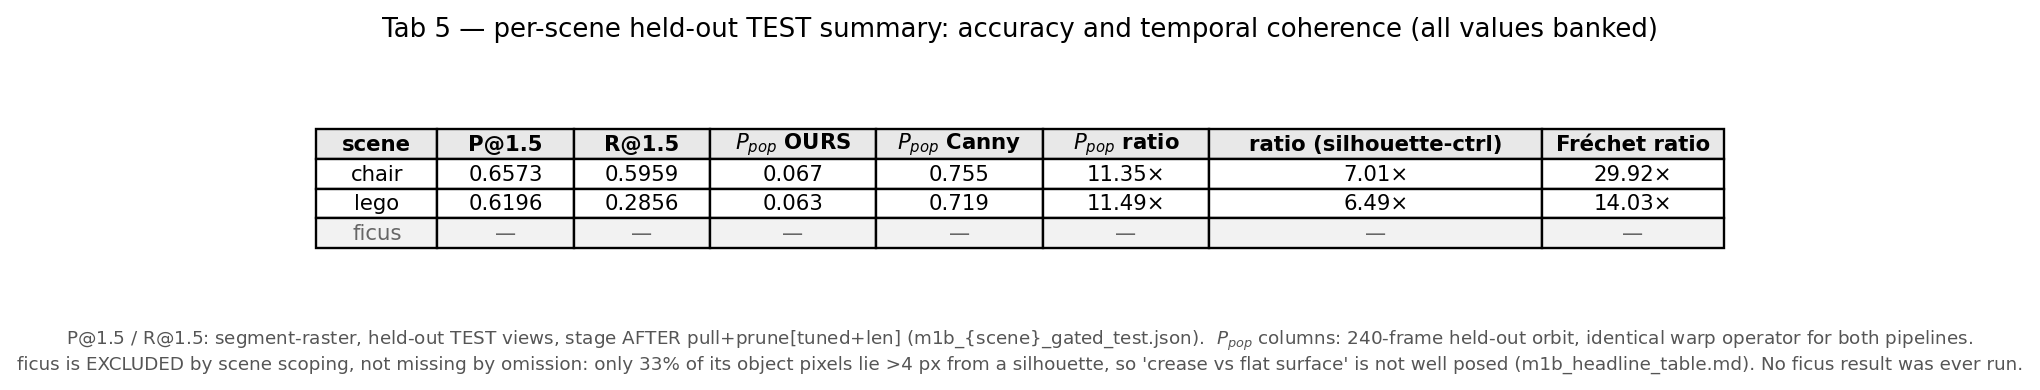
\includegraphics[width=0.82\textwidth]{assets/tab5_per_scene.png}\end{table*}


\clearpage
\appendices
\section{Can a discriminator patch the boundary? A pre-emptive falsification}
\emph{(All numbers from \texttt{RESULTS\_MASTER.md} \S4, sourced in \texttt{phase1e\_test\_eval.json},
\texttt{phase1e\_scores\_meta.json}, \texttt{phase1f\_test\_eval.json}, plus banked ledger numbers
quoted unchanged; full protocol and caveats in \texttt{PHASE1E\_GATE\_CHECK.md} /
\texttt{PHASE1F\_CHAIN\_GATE.md}.)}

The natural reviewer objection to \S5 is operational: \emph{"the crease-vs-texture signal
exists (0.8401/0.9044) --- why not just train a lightweight discriminator, or pool it over
chains, and filter the texture edges out?"} We ran that experiment, both ways, before a
reviewer could ask --- as two post-lock falsification probes under the paper's own
discipline: thresholds frozen on VAL views only, TEST evaluated exactly once per arm, and
the method-path invariant intact (every gate SCORE is mesh-free at the target scene; the
in-scene mesh-supervised probe appears only as a labelled oracle upper bound, never as a
result). The candidate set is the Phase-1b chair triangulated cloud (272,366 points), and
the metric is the same macro segment-raster P@1.5px convention as the pipeline baseline
it must beat (0.6573 at recall 0.5959, quoted from its banked run, never re-run).

\textbf{A.1 Mesh-free gating converts nothing (the supervision barrier, at the cloud level).}
The only deployment-legal transfer discriminator at chair --- fit on the \emph{other} scene's
mesh labels --- carries AUC 0.5626 (chance; \S5.4's 0.8245 is the \emph{reverse} direction, fit
on chair's own mesh, and is therefore not legal as a chair gate). Gated at matched
recall, it moves precision from 0.3189 (ungated) to 0.3216. The best in-scene mesh-free
gate (the physics-frozen geometric-photometric vote of \S5.4) reaches \textbf{0.4458} at recall
0.6156 --- far under both the 0.6573 baseline and the probes' frozen 0.71 GO bar --- and
already breaks crease connectivity (topology guard 0.8811, bar 0.90). NO-GO, with margin.

\textbf{A.2 Even the oracle cannot filter its way through (the topological trilemma).} The
same cloud gated by an in-scene \emph{mesh-supervised} probe (in-sample AUC 0.9578 --- the
loosest possible upper bound, and mesh-in-the-loop, so an oracle by construction) reaches
P@1.5 \textbf{0.7970} at matched recall --- and retains only \textbf{0.6372} of the
baseline-covered GT crease segments: per-point selection drops the low-scoring bridge
points that keep 1D chains connected. Chain-mean pooling --- the reviewer's fix, run
exactly as proposed on the label-pure chain structure of \S5.3 (1,692 components) ---
repairs part of that (guard 0.6372 $\rightarrow$ 0.7481 mean-pooled, 0.7970 median-pooled) at a real
precision cost (point-oracle 0.7970 $\rightarrow$ chain-gated 0.6458, \emph{below} the 0.6573 baseline),
and its ceiling is structural: keeping \textbf{every} chain with
no thresholding at all already caps the guard at \textbf{0.8782 < 0.90}, because the 42.36 \%
of candidates no proximity+direction chain absorbs are precisely the bridging points.
Across every tested gate --- mesh-free or oracle, point-gated or chain-pooled --- no
tested operating point attains precision $\geq$ 0.71, recall $\geq$ the baseline's 0.5959, and
topology $\geq$ 0.90 \emph{simultaneously}. That is the trilemma, and it is a property of the
repair class: post-hoc keep/drop filtering of a fixed candidate cloud trades precision
against 1D continuity for every ranking we could construct, up to an in-sample oracle.
The oracle also bounds the class: any learned gate's ranking on this fixed cloud is
dominated by the in-sample oracle, so the trilemma binds post-hoc discriminator gating
as a \emph{class}, not merely the gates we built.

\textbf{A.3 What this hardens.} Two independent barriers now stand between the cloud and a
deployable precision fix: the supervision gap (mesh-free discrimination is chance-level
where it is legal, \S5.4 and A.1) and the continuity severing (even oracle ranking cannot
threshold without fragmenting chains, A.2). Fixing either alone is measurably
insufficient; a build that wanted this precision would need \emph{topology-aware
construction} --- connectivity as a constraint during line formation, not a casualty of
filtering after it --- plus labeled scenes. This is why \S5's boundary ships as a measured
boundary: the obvious patches are not merely unattempted, they are falsified. Probe
scope, disclosed: cloud-level results are chair-only (n=1 scene) --- chair being the
deliberately selected texture-stress case (Canny edge purity 0.28), so the repair class
was falsified on its adversarial home ground, no scene-independent impossibility is
claimed, and extending the falsification beyond chair is named future work; the oracle
bound is
in-sample (loosest); the cloud is rasterised as points inside the segment-raster
convention (its 272k points saturate recall at 0.9540 ungated, so the NO-GO is not a
rasterisation artifact).

\textbf{A.4 A learned line field cannot escape the boundary either (the epipolar accumulation
test).} \emph{(Numbers from \texttt{EPIPOLAR\_ACCUM\_RESULTS.md}; script \texttt{scripts/epi\_accum.py},
arrays \texttt{out/epi/}. Mesh EVAL-ONLY: it supplies the two label sets and the visibility
of their points; the accumulated feature is mesh-free.)} The remaining objection is
representational: a dedicated 3D edge field, trained on the detector's multi-view 2D edge
maps and combined with the frozen 3DGS for occlusion, might integrate sub-threshold
evidence coherently across views and so recover creases that per-view thresholding
misses. Any such field, whatever its architecture, can learn at most what its
multi-view projection loss can see; the closed-form upper bound of that loss is the
occlusion-aware multi-view mean $\bar{S}$ of the \emph{raw} detector probability at the true 3D
location. We evaluated $\bar{S}$ on the GT creases the frozen pipeline misses (lego 437,138
points, chair 73,371 --- the pre-registered miss-set of the coverage analysis) against an
equal number of genuinely flat GT surface points (farther than 3 px, twice the scoring
tolerance, from any geometric $\geq$10$^{\circ}$ edge, boundary edge, or non-manifold edge of the
position-merged mesh; visible in $\geq$1 held-out view under the same mesh-depth rule), over
all 100 views, with occlusion from the frozen 3DGS z-buffer under the pipeline's own
tolerance, using DexiNed's raw sigmoid maps (never thresholded; continuity asserted at
run time) and the pipeline's half-pixel convention, calibrated on the recovered creases.
Gate, frozen before any number: GO iff AUC $\geq$ 0.80 and recall $\geq$ 0.55 at 85 \% precision;
NO-GO iff AUC $\leq$ 0.65 or that recall $\leq$ 0.42.

Result: \textbf{lego AUC 0.698, recall at 85 \% precision 0.000; chair 0.859 / 0.000 --- NO-GO on
both scenes.} The single-view baseline (the same points scored in one view, balanced)
reaches AUC 0.644 / 0.738 (best views 0.758 / 0.828); the paired multi-view lift is
+0.049 (lego) / +0.133 (chair) AUC --- real, but it does not reach the recall criterion.
Two readings the numbers rule out. (i) \emph{Dead zeros}: only 11 \% of lego's missed creases
are undetected by the pipeline's own rule in every visible view (they are true dead
zeros, $\bar{S}$ median 0.010); the other 89 \% are detected somewhere and score AUC 0.76 against
flat surface. (ii) \emph{An over-strict negative class}: the flat set's distance to the nearest
geometric edge sweeps the criterion continuously --- $\bar{S}$ on flat surface is 0.136 at 3--4 px,
0.097 at 4--5 px, 0.073 at 5--6 px, 0.036 at 8--12 px (missed creases 0.220) --- i.e. the
detector's response tail reaches $\approx$5 px, and 83 \% of lego's flat surface lies within 4.5 px
of an edge (97 \% within 6 px). Widening the margin lets the criterion pass (lego 6 px:
AUC 0.831, recall 0.665) only by restricting the negative class to the 3 \% of the surface
that is farther from any edge than the detector's footprint --- which is not the surface a
line field must reject. On chair the zero recall is a knife-edge (removing the 1,000
highest-scoring flat points --- 1.4 \%, on rails that are silhouettes in most views --- lifts
it to 0.53); on lego it is structural (removing 5,000 lifts it to 0.055). The kill
mechanism is therefore the spatial resolution of the 2D supervision on an edge-dense
surface, not missing signal, and it binds any field trained on that supervision. All
mesh-free analysis choices (native/multi-scale maps, bilinear/1.5 px-max sampling, two
occlusion tolerances, 100 or 80 views, mean/median/trimmed/logit/max aggregation, a 3 px
silhouette peel) leave lego's best AUC at 0.713 and its recall at 85 \% precision below
0.004; the headline numbers were reproduced to $10^{-9}$ by an independent re-computation
from the saved arrays. A first run of this test with a flat set built from the
split-vertex adjacency (the topology issue of A.5) read 0.572 / 0.733 and is superseded.

\textbf{A.5 The ground-truth crease set is a topology-selected subset.} The crease set is
built from face adjacency of the mesh as loaded from the asset file, and the
NeRF-synthetic OBJs store split vertices (one per position/texture/normal triplet): a
hard-shaded crease or a UV seam is therefore an \emph{open-boundary} edge with no face
adjacency and is absent from the crease set. Measured on position-merged copies of the
meshes, the crease set used throughout covers \textbf{37 \% (lego) / 43 \% (chair) / 31 \% (ficus)}
of the geometric $\geq$30$^{\circ}$ edges, and none of a plant's open leaf rims; every precision/recall
number in this paper --- ours and every baseline's --- is scored against that subset. The
subset does not flatter the ceiling: on the full geometric crease set the frozen
multi-view triangulation of \S5.2 recovers 0.175 (lego) / 0.598 (chair) of visible
creases, with the never-counted creases slightly \emph{harder} (0.159 / 0.545) than the counted
ones (0.199 / 0.665), so the coverage conclusions stand; the absolute recall values are
definition-specific and are always to be quoted with it.



\end{document}
